\documentclass{book}
\usepackage[a4paper,top=2.5cm,bottom=2.5cm,left=2.5cm,right=2.5cm]{geometry}
\usepackage{makeidx}
\usepackage{natbib}
\usepackage{graphicx}
\usepackage{multicol}
\usepackage{float}
\usepackage{listings}
\usepackage{color}
\usepackage{ifthen}
\usepackage[table]{xcolor}
\usepackage{textcomp}
\usepackage{alltt}
\usepackage{ifpdf}
\ifpdf
\usepackage[pdftex,
            pagebackref=true,
            colorlinks=true,
            linkcolor=blue,
            unicode
           ]{hyperref}
\else
\usepackage[ps2pdf,
            pagebackref=true,
            colorlinks=true,
            linkcolor=blue,
            unicode
           ]{hyperref}
\usepackage{pspicture}
\fi
\usepackage[utf8]{inputenc}
\usepackage{mathptmx}
\usepackage[scaled=.90]{helvet}
\usepackage{courier}
\usepackage{sectsty}
\usepackage{amssymb}
\usepackage[titles]{tocloft}
\usepackage{doxygen}
\lstset{language=C++,inputencoding=utf8,basicstyle=\footnotesize,breaklines=true,breakatwhitespace=true,tabsize=1,numbers=left }
\makeindex
\setcounter{tocdepth}{3}
\renewcommand{\footrulewidth}{0.4pt}
\renewcommand{\familydefault}{\sfdefault}
\hfuzz=15pt
\setlength{\emergencystretch}{15pt}
\hbadness=750
\tolerance=750
\begin{document}
\hypersetup{pageanchor=false,citecolor=blue}
\begin{titlepage}
\vspace*{7cm}
\begin{center}
{\Large G\-E\-A\-N\-T4 Simulation \\[1ex]\large version 0.\-5 (January 9th, 2013) }\\
\vspace*{1cm}
{\large Generated by Doxygen 1.8.2}\\
\vspace*{0.5cm}
{\small Wed Jan 9 2013 14:26:39}\\
\end{center}
\end{titlepage}
\clearemptydoublepage
\pagenumbering{roman}
\tableofcontents
\clearemptydoublepage
\pagenumbering{arabic}
\hypersetup{pageanchor=true,citecolor=blue}
\chapter{Hierarchical Index}
\section{Class Hierarchy}
This inheritance list is sorted roughly, but not completely, alphabetically\-:\begin{DoxyCompactList}
\item G4\-Run\begin{DoxyCompactList}
\item \contentsline{section}{Run}{\pageref{class_run}}{}
\end{DoxyCompactList}
\item G4\-User\-Run\-Action\begin{DoxyCompactList}
\item \contentsline{section}{Run\-Action}{\pageref{class_run_action}}{}
\item \contentsline{section}{Teste\-User\-Run\-Action}{\pageref{class_teste_user_run_action}}{}
\end{DoxyCompactList}
\item G4\-V\-User\-Detector\-Construction\begin{DoxyCompactList}
\item \contentsline{section}{Detector\-Construction}{\pageref{class_detector_construction}}{}
\item \contentsline{section}{Teste\-Detector\-Construction}{\pageref{class_teste_detector_construction}}{}
\end{DoxyCompactList}
\item G4\-V\-User\-Physics\-List\begin{DoxyCompactList}
\item \contentsline{section}{Physics\-List}{\pageref{class_physics_list}}{}
\item \contentsline{section}{Physics\-List}{\pageref{class_physics_list}}{}
\item \contentsline{section}{Teste\-Physics\-List}{\pageref{class_teste_physics_list}}{}
\end{DoxyCompactList}
\item G4\-V\-User\-Primary\-Generator\-Action\begin{DoxyCompactList}
\item \contentsline{section}{Primary\-Generator\-Action}{\pageref{class_primary_generator_action}}{}
\item \contentsline{section}{Teste\-Primary\-Generator\-Action}{\pageref{class_teste_primary_generator_action}}{}
\end{DoxyCompactList}
\item \contentsline{section}{My\-Material}{\pageref{class_my_material}}{}
\item \contentsline{section}{My\-Random}{\pageref{class_my_random}}{}
\item \contentsline{section}{Teste}{\pageref{class_teste}}{}
\end{DoxyCompactList}

\chapter{Class Index}
\section{Class List}
Here are the classes, structs, unions and interfaces with brief descriptions\-:\begin{DoxyCompactList}
\item\contentsline{section}{\hyperlink{class_detector_construction}{Detector\-Construction} }{\pageref{class_detector_construction}}{}
\item\contentsline{section}{\hyperlink{class_my_material}{My\-Material} }{\pageref{class_my_material}}{}
\item\contentsline{section}{\hyperlink{class_my_random}{My\-Random} }{\pageref{class_my_random}}{}
\item\contentsline{section}{\hyperlink{class_physics_list}{Physics\-List} }{\pageref{class_physics_list}}{}
\item\contentsline{section}{\hyperlink{class_primary_generator_action}{Primary\-Generator\-Action} }{\pageref{class_primary_generator_action}}{}
\item\contentsline{section}{\hyperlink{class_run}{Run} }{\pageref{class_run}}{}
\item\contentsline{section}{\hyperlink{class_run_action}{Run\-Action} }{\pageref{class_run_action}}{}
\item\contentsline{section}{\hyperlink{class_teste}{Teste} }{\pageref{class_teste}}{}
\item\contentsline{section}{\hyperlink{class_teste_detector_construction}{Teste\-Detector\-Construction} }{\pageref{class_teste_detector_construction}}{}
\item\contentsline{section}{\hyperlink{class_teste_physics_list}{Teste\-Physics\-List} }{\pageref{class_teste_physics_list}}{}
\item\contentsline{section}{\hyperlink{class_teste_primary_generator_action}{Teste\-Primary\-Generator\-Action} }{\pageref{class_teste_primary_generator_action}}{}
\item\contentsline{section}{\hyperlink{class_teste_user_run_action}{Teste\-User\-Run\-Action} }{\pageref{class_teste_user_run_action}}{}
\end{DoxyCompactList}

\chapter{File Index}
\section{File List}
Here is a list of all files with brief descriptions\-:\begin{DoxyCompactList}
\item\contentsline{section}{\hyperlink{_detector_construction_8cc}{Detector\-Construction.\-cc} }{\pageref{_detector_construction_8cc}}{}
\item\contentsline{section}{\hyperlink{_detector_construction_8hh}{Detector\-Construction.\-hh} }{\pageref{_detector_construction_8hh}}{}
\item\contentsline{section}{\hyperlink{_geant4_master_dissertation_simulation_8cc}{Geant4\-Master\-Dissertation\-Simulation.\-cc} }{\pageref{_geant4_master_dissertation_simulation_8cc}}{}
\item\contentsline{section}{\hyperlink{_my_material_8cc}{My\-Material.\-cc} }{\pageref{_my_material_8cc}}{}
\item\contentsline{section}{\hyperlink{_my_material_8hh}{My\-Material.\-hh} }{\pageref{_my_material_8hh}}{}
\item\contentsline{section}{\hyperlink{_my_random_8cc}{My\-Random.\-cc} }{\pageref{_my_random_8cc}}{}
\item\contentsline{section}{\hyperlink{_my_random_8hh}{My\-Random.\-hh} }{\pageref{_my_random_8hh}}{}
\item\contentsline{section}{\hyperlink{src_2_physics_list_8cc}{src/\-Physics\-List.\-cc} }{\pageref{src_2_physics_list_8cc}}{}
\item\contentsline{section}{\hyperlink{stuff_2_physics_list_8cc}{stuff/\-Physics\-List.\-cc} }{\pageref{stuff_2_physics_list_8cc}}{}
\item\contentsline{section}{\hyperlink{include_2_physics_list_8hh}{include/\-Physics\-List.\-hh} }{\pageref{include_2_physics_list_8hh}}{}
\item\contentsline{section}{\hyperlink{stuff_2_physics_list_8hh}{stuff/\-Physics\-List.\-hh} }{\pageref{stuff_2_physics_list_8hh}}{}
\item\contentsline{section}{\hyperlink{_primary_generator_action_8cc}{Primary\-Generator\-Action.\-cc} }{\pageref{_primary_generator_action_8cc}}{}
\item\contentsline{section}{\hyperlink{_primary_generator_action_8hh}{Primary\-Generator\-Action.\-hh} }{\pageref{_primary_generator_action_8hh}}{}
\item\contentsline{section}{\hyperlink{_run_8cc}{Run.\-cc} }{\pageref{_run_8cc}}{}
\item\contentsline{section}{\hyperlink{_run_8hh}{Run.\-hh} }{\pageref{_run_8hh}}{}
\item\contentsline{section}{\hyperlink{src_2_run_action_8cc}{src/\-Run\-Action.\-cc} }{\pageref{src_2_run_action_8cc}}{}
\item\contentsline{section}{\hyperlink{stuff_2_run_action_8cc}{stuff/\-Run\-Action.\-cc} }{\pageref{stuff_2_run_action_8cc}}{}
\item\contentsline{section}{\hyperlink{_run_action_8hh}{Run\-Action.\-hh} }{\pageref{_run_action_8hh}}{}
\item\contentsline{section}{\hyperlink{_teste_8cc}{Teste.\-cc} }{\pageref{_teste_8cc}}{}
\item\contentsline{section}{\hyperlink{_teste_8hh}{Teste.\-hh} }{\pageref{_teste_8hh}}{}
\item\contentsline{section}{\hyperlink{_teste_detector_construction_8cc}{Teste\-Detector\-Construction.\-cc} }{\pageref{_teste_detector_construction_8cc}}{}
\item\contentsline{section}{\hyperlink{_teste_detector_construction_8hh}{Teste\-Detector\-Construction.\-hh} }{\pageref{_teste_detector_construction_8hh}}{}
\item\contentsline{section}{\hyperlink{_teste_physics_list_8cc}{Teste\-Physics\-List.\-cc} }{\pageref{_teste_physics_list_8cc}}{}
\item\contentsline{section}{\hyperlink{_teste_physics_list_8hh}{Teste\-Physics\-List.\-hh} }{\pageref{_teste_physics_list_8hh}}{}
\item\contentsline{section}{\hyperlink{_teste_primary_generator_action_8cc}{Teste\-Primary\-Generator\-Action.\-cc} }{\pageref{_teste_primary_generator_action_8cc}}{}
\item\contentsline{section}{\hyperlink{_teste_primary_generator_action_8hh}{Teste\-Primary\-Generator\-Action.\-hh} }{\pageref{_teste_primary_generator_action_8hh}}{}
\item\contentsline{section}{\hyperlink{_teste_user_run_action_8cc}{Teste\-User\-Run\-Action.\-cc} }{\pageref{_teste_user_run_action_8cc}}{}
\item\contentsline{section}{\hyperlink{_teste_user_run_action_8hh}{Teste\-User\-Run\-Action.\-hh} }{\pageref{_teste_user_run_action_8hh}}{}
\end{DoxyCompactList}

\chapter{Class Documentation}
\hypertarget{class_detector_construction}{\section{Detector\-Construction Class Reference}
\label{class_detector_construction}\index{Detector\-Construction@{Detector\-Construction}}
}


{\ttfamily \#include $<$Detector\-Construction.\-hh$>$}

Inheritance diagram for Detector\-Construction\-:\begin{figure}[H]
\begin{center}
\leavevmode
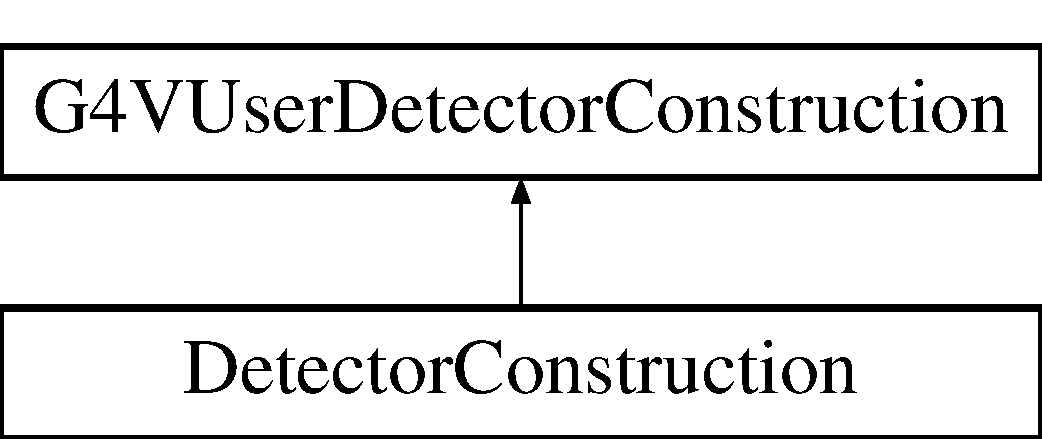
\includegraphics[height=2.000000cm]{class_detector_construction}
\end{center}
\end{figure}
\subsection*{Public Member Functions}
\begin{DoxyCompactItemize}
\item 
\hyperlink{class_detector_construction_a1533c4308baddd0b2dcdf40f61dea1ef}{Detector\-Construction} ()
\item 
\hyperlink{class_detector_construction_a73013cab35a2b470338da2e4686edea3}{$\sim$\-Detector\-Construction} ()
\item 
G4\-V\-Physical\-Volume $\ast$ \hyperlink{class_detector_construction_a662c618480b345a747f014b845d5ffdf}{Construct} ()
\item 
G4\-V\-Physical\-Volume $\ast$ \hyperlink{class_detector_construction_ab3d0fbcccb1be35f505a78e7fd4ffce2}{get\-Word\-Volume} ()
\item 
G4\-V\-Physical\-Volume $\ast$ \hyperlink{class_detector_construction_af45ab5e73219e233c7c015573cf4f88f}{get\-Cube} ()
\end{DoxyCompactItemize}


\subsection{Detailed Description}


Definition at line 16 of file Detector\-Construction.\-hh.



\subsection{Constructor \& Destructor Documentation}
\hypertarget{class_detector_construction_a1533c4308baddd0b2dcdf40f61dea1ef}{\index{Detector\-Construction@{Detector\-Construction}!Detector\-Construction@{Detector\-Construction}}
\index{Detector\-Construction@{Detector\-Construction}!DetectorConstruction@{Detector\-Construction}}
\subsubsection[{Detector\-Construction}]{\setlength{\rightskip}{0pt plus 5cm}Detector\-Construction\-::\-Detector\-Construction (
\begin{DoxyParamCaption}
{}
\end{DoxyParamCaption}
)}}\label{class_detector_construction_a1533c4308baddd0b2dcdf40f61dea1ef}
\begin{DoxyAuthor}{Author}
Sandro Boschetti, August 30, 2012 
\end{DoxyAuthor}


Definition at line 27 of file Detector\-Construction.\-cc.

\hypertarget{class_detector_construction_a73013cab35a2b470338da2e4686edea3}{\index{Detector\-Construction@{Detector\-Construction}!$\sim$\-Detector\-Construction@{$\sim$\-Detector\-Construction}}
\index{$\sim$\-Detector\-Construction@{$\sim$\-Detector\-Construction}!DetectorConstruction@{Detector\-Construction}}
\subsubsection[{$\sim$\-Detector\-Construction}]{\setlength{\rightskip}{0pt plus 5cm}Detector\-Construction\-::$\sim$\-Detector\-Construction (
\begin{DoxyParamCaption}
{}
\end{DoxyParamCaption}
)}}\label{class_detector_construction_a73013cab35a2b470338da2e4686edea3}


Definition at line 32 of file Detector\-Construction.\-cc.



\subsection{Member Function Documentation}
\hypertarget{class_detector_construction_a662c618480b345a747f014b845d5ffdf}{\index{Detector\-Construction@{Detector\-Construction}!Construct@{Construct}}
\index{Construct@{Construct}!DetectorConstruction@{Detector\-Construction}}
\subsubsection[{Construct}]{\setlength{\rightskip}{0pt plus 5cm}G4\-V\-Physical\-Volume $\ast$ Detector\-Construction\-::\-Construct (
\begin{DoxyParamCaption}
{}
\end{DoxyParamCaption}
)}}\label{class_detector_construction_a662c618480b345a747f014b845d5ffdf}
A Logical\-Volume is some geometry figure, like a G4\-Box, fulfilled with some material.

A Physical\-Volume is a Logical\-Volume put in place.

Here I set the Sensitive Detector used to accumulate radiation dose. There is a bunch of things that must be U\-N\-D\-E\-R\-S\-T\-O\-O\-D here.

Definition at line 45 of file Detector\-Construction.\-cc.

\hypertarget{class_detector_construction_af45ab5e73219e233c7c015573cf4f88f}{\index{Detector\-Construction@{Detector\-Construction}!get\-Cube@{get\-Cube}}
\index{get\-Cube@{get\-Cube}!DetectorConstruction@{Detector\-Construction}}
\subsubsection[{get\-Cube}]{\setlength{\rightskip}{0pt plus 5cm}G4\-V\-Physical\-Volume $\ast$ Detector\-Construction\-::get\-Cube (
\begin{DoxyParamCaption}
{}
\end{DoxyParamCaption}
)}}\label{class_detector_construction_af45ab5e73219e233c7c015573cf4f88f}


Definition at line 41 of file Detector\-Construction.\-cc.

\hypertarget{class_detector_construction_ab3d0fbcccb1be35f505a78e7fd4ffce2}{\index{Detector\-Construction@{Detector\-Construction}!get\-Word\-Volume@{get\-Word\-Volume}}
\index{get\-Word\-Volume@{get\-Word\-Volume}!DetectorConstruction@{Detector\-Construction}}
\subsubsection[{get\-Word\-Volume}]{\setlength{\rightskip}{0pt plus 5cm}G4\-V\-Physical\-Volume $\ast$ Detector\-Construction\-::get\-Word\-Volume (
\begin{DoxyParamCaption}
{}
\end{DoxyParamCaption}
)}}\label{class_detector_construction_ab3d0fbcccb1be35f505a78e7fd4ffce2}


Definition at line 37 of file Detector\-Construction.\-cc.



The documentation for this class was generated from the following files\-:\begin{DoxyCompactItemize}
\item 
\hyperlink{_detector_construction_8hh}{Detector\-Construction.\-hh}\item 
\hyperlink{_detector_construction_8cc}{Detector\-Construction.\-cc}\end{DoxyCompactItemize}

\hypertarget{class_my_material}{\section{My\-Material Class Reference}
\label{class_my_material}\index{My\-Material@{My\-Material}}
}


{\ttfamily \#include $<$My\-Material.\-hh$>$}

\subsection*{Public Member Functions}
\begin{DoxyCompactItemize}
\item 
\hyperlink{class_my_material_a6dfecac02071e92badb081ce71f9ab59}{My\-Material} ()
\item 
virtual \hyperlink{class_my_material_a2b1fc5dcf2728e33f31f8593da92fae4}{$\sim$\-My\-Material} ()
\item 
G4\-Material $\ast$ \hyperlink{class_my_material_a44363a322d66a290c958cd0f91a81677}{get\-Air} ()
\item 
G4\-Material $\ast$ \hyperlink{class_my_material_a8f3b8a3613e513e63d4d96cdcd848780}{get\-Argon\-Gas} ()
\item 
G4\-Material $\ast$ \hyperlink{class_my_material_a3241e5b639f4bc47aa4c6671f3934bd0}{get\-Pb} ()
\item 
G4\-Material $\ast$ \hyperlink{class_my_material_a4b60ce3a99c596c162d33d2afe3d6813}{get\-Water} ()
\end{DoxyCompactItemize}


\subsection{Detailed Description}


Definition at line 12 of file My\-Material.\-hh.



\subsection{Constructor \& Destructor Documentation}
\hypertarget{class_my_material_a6dfecac02071e92badb081ce71f9ab59}{\index{My\-Material@{My\-Material}!My\-Material@{My\-Material}}
\index{My\-Material@{My\-Material}!MyMaterial@{My\-Material}}
\subsubsection[{My\-Material}]{\setlength{\rightskip}{0pt plus 5cm}My\-Material\-::\-My\-Material (
\begin{DoxyParamCaption}
{}
\end{DoxyParamCaption}
)}}\label{class_my_material_a6dfecac02071e92badb081ce71f9ab59}


Definition at line 12 of file My\-Material.\-cc.

\hypertarget{class_my_material_a2b1fc5dcf2728e33f31f8593da92fae4}{\index{My\-Material@{My\-Material}!$\sim$\-My\-Material@{$\sim$\-My\-Material}}
\index{$\sim$\-My\-Material@{$\sim$\-My\-Material}!MyMaterial@{My\-Material}}
\subsubsection[{$\sim$\-My\-Material}]{\setlength{\rightskip}{0pt plus 5cm}My\-Material\-::$\sim$\-My\-Material (
\begin{DoxyParamCaption}
{}
\end{DoxyParamCaption}
)\hspace{0.3cm}{\ttfamily [virtual]}}}\label{class_my_material_a2b1fc5dcf2728e33f31f8593da92fae4}


Definition at line 43 of file My\-Material.\-cc.



\subsection{Member Function Documentation}
\hypertarget{class_my_material_a44363a322d66a290c958cd0f91a81677}{\index{My\-Material@{My\-Material}!get\-Air@{get\-Air}}
\index{get\-Air@{get\-Air}!MyMaterial@{My\-Material}}
\subsubsection[{get\-Air}]{\setlength{\rightskip}{0pt plus 5cm}G4\-Material $\ast$ My\-Material\-::get\-Air (
\begin{DoxyParamCaption}
{}
\end{DoxyParamCaption}
)}}\label{class_my_material_a44363a322d66a290c958cd0f91a81677}


Definition at line 47 of file My\-Material.\-cc.

\hypertarget{class_my_material_a8f3b8a3613e513e63d4d96cdcd848780}{\index{My\-Material@{My\-Material}!get\-Argon\-Gas@{get\-Argon\-Gas}}
\index{get\-Argon\-Gas@{get\-Argon\-Gas}!MyMaterial@{My\-Material}}
\subsubsection[{get\-Argon\-Gas}]{\setlength{\rightskip}{0pt plus 5cm}G4\-Material $\ast$ My\-Material\-::get\-Argon\-Gas (
\begin{DoxyParamCaption}
{}
\end{DoxyParamCaption}
)}}\label{class_my_material_a8f3b8a3613e513e63d4d96cdcd848780}


Definition at line 51 of file My\-Material.\-cc.

\hypertarget{class_my_material_a3241e5b639f4bc47aa4c6671f3934bd0}{\index{My\-Material@{My\-Material}!get\-Pb@{get\-Pb}}
\index{get\-Pb@{get\-Pb}!MyMaterial@{My\-Material}}
\subsubsection[{get\-Pb}]{\setlength{\rightskip}{0pt plus 5cm}G4\-Material $\ast$ My\-Material\-::get\-Pb (
\begin{DoxyParamCaption}
{}
\end{DoxyParamCaption}
)}}\label{class_my_material_a3241e5b639f4bc47aa4c6671f3934bd0}


Definition at line 55 of file My\-Material.\-cc.

\hypertarget{class_my_material_a4b60ce3a99c596c162d33d2afe3d6813}{\index{My\-Material@{My\-Material}!get\-Water@{get\-Water}}
\index{get\-Water@{get\-Water}!MyMaterial@{My\-Material}}
\subsubsection[{get\-Water}]{\setlength{\rightskip}{0pt plus 5cm}G4\-Material $\ast$ My\-Material\-::get\-Water (
\begin{DoxyParamCaption}
{}
\end{DoxyParamCaption}
)}}\label{class_my_material_a4b60ce3a99c596c162d33d2afe3d6813}


Definition at line 59 of file My\-Material.\-cc.



The documentation for this class was generated from the following files\-:\begin{DoxyCompactItemize}
\item 
\hyperlink{_my_material_8hh}{My\-Material.\-hh}\item 
\hyperlink{_my_material_8cc}{My\-Material.\-cc}\end{DoxyCompactItemize}

\hypertarget{class_my_random}{\section{My\-Random Class Reference}
\label{class_my_random}\index{My\-Random@{My\-Random}}
}


{\ttfamily \#include $<$My\-Random.\-hh$>$}

\subsection*{Public Member Functions}
\begin{DoxyCompactItemize}
\item 
double \hyperlink{class_my_random_a9a10d5547334be89143a134192b982e0}{get\-Random\-Number} ()
\item 
\hyperlink{class_my_random_a1d81672232fc7045199587ffe1102044}{My\-Random} ()
\item 
virtual \hyperlink{class_my_random_abdfe9d5ec4fd9a6d78637d618aee9ca3}{$\sim$\-My\-Random} ()
\end{DoxyCompactItemize}


\subsection{Detailed Description}


Definition at line 21 of file My\-Random.\-hh.



\subsection{Constructor \& Destructor Documentation}
\hypertarget{class_my_random_a1d81672232fc7045199587ffe1102044}{\index{My\-Random@{My\-Random}!My\-Random@{My\-Random}}
\index{My\-Random@{My\-Random}!MyRandom@{My\-Random}}
\subsubsection[{My\-Random}]{\setlength{\rightskip}{0pt plus 5cm}My\-Random\-::\-My\-Random (
\begin{DoxyParamCaption}
{}
\end{DoxyParamCaption}
)}}\label{class_my_random_a1d81672232fc7045199587ffe1102044}


Definition at line 8 of file My\-Random.\-cc.

\hypertarget{class_my_random_abdfe9d5ec4fd9a6d78637d618aee9ca3}{\index{My\-Random@{My\-Random}!$\sim$\-My\-Random@{$\sim$\-My\-Random}}
\index{$\sim$\-My\-Random@{$\sim$\-My\-Random}!MyRandom@{My\-Random}}
\subsubsection[{$\sim$\-My\-Random}]{\setlength{\rightskip}{0pt plus 5cm}My\-Random\-::$\sim$\-My\-Random (
\begin{DoxyParamCaption}
{}
\end{DoxyParamCaption}
)\hspace{0.3cm}{\ttfamily [virtual]}}}\label{class_my_random_abdfe9d5ec4fd9a6d78637d618aee9ca3}


Definition at line 13 of file My\-Random.\-cc.



\subsection{Member Function Documentation}
\hypertarget{class_my_random_a9a10d5547334be89143a134192b982e0}{\index{My\-Random@{My\-Random}!get\-Random\-Number@{get\-Random\-Number}}
\index{get\-Random\-Number@{get\-Random\-Number}!MyRandom@{My\-Random}}
\subsubsection[{get\-Random\-Number}]{\setlength{\rightskip}{0pt plus 5cm}double My\-Random\-::get\-Random\-Number (
\begin{DoxyParamCaption}
{}
\end{DoxyParamCaption}
)}}\label{class_my_random_a9a10d5547334be89143a134192b982e0}


Definition at line 3 of file My\-Random.\-cc.



The documentation for this class was generated from the following files\-:\begin{DoxyCompactItemize}
\item 
\hyperlink{_my_random_8hh}{My\-Random.\-hh}\item 
\hyperlink{_my_random_8cc}{My\-Random.\-cc}\end{DoxyCompactItemize}

\hypertarget{class_physics_list}{\section{Physics\-List Class Reference}
\label{class_physics_list}\index{Physics\-List@{Physics\-List}}
}


{\ttfamily \#include $<$Physics\-List.\-hh$>$}

Inheritance diagram for Physics\-List\-:\begin{figure}[H]
\begin{center}
\leavevmode
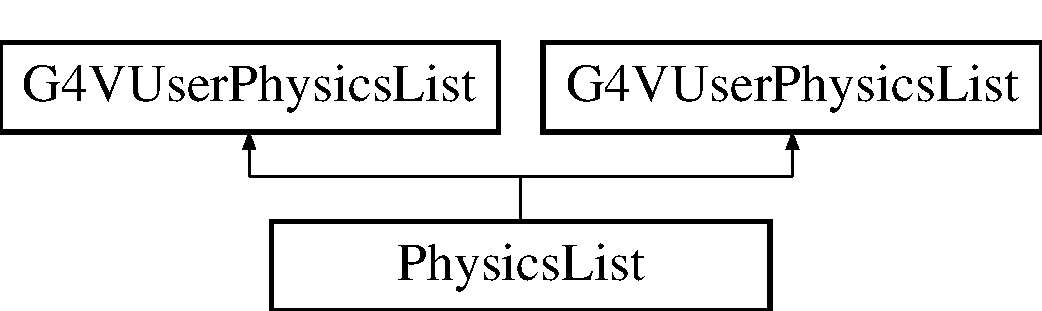
\includegraphics[height=2.000000cm]{class_physics_list}
\end{center}
\end{figure}
\subsection*{Public Member Functions}
\begin{DoxyCompactItemize}
\item 
\hyperlink{class_physics_list_aeecf835245a0b10c24e5e6c37cbb0dab}{Physics\-List} ()
\item 
\hyperlink{class_physics_list_a6cff761e006f8d5c57f0beca0e7d61ae}{$\sim$\-Physics\-List} ()
\item 
\hyperlink{class_physics_list_aeecf835245a0b10c24e5e6c37cbb0dab}{Physics\-List} ()
\item 
\hyperlink{class_physics_list_a6cff761e006f8d5c57f0beca0e7d61ae}{$\sim$\-Physics\-List} ()
\end{DoxyCompactItemize}
\subsection*{Protected Member Functions}
\begin{DoxyCompactItemize}
\item 
void \hyperlink{class_physics_list_af7906507122c985d2da3e61c56efe60e}{Construct\-Particle} ()
\item 
void \hyperlink{class_physics_list_a9c08bc28eba2ae62104b967280901a3f}{Construct\-Process} ()
\item 
void \hyperlink{class_physics_list_a0ba901b82ae30657b109930645fe8017}{Set\-Cuts} ()
\item 
void \hyperlink{class_physics_list_ab7158dbb73a310fc99331005277502b5}{Construct\-Bosons} ()
\item 
void \hyperlink{class_physics_list_ab55f046b278d5c02b8c83aaa332504ec}{Construct\-Leptons} ()
\item 
void \hyperlink{class_physics_list_a2d4d082da733c65153a801a7c70a276e}{Construct\-Mesons} ()
\item 
void \hyperlink{class_physics_list_a628054b8fcfbd759d3f1a65b1eba7e01}{Construct\-Baryons} ()
\item 
void \hyperlink{class_physics_list_a413551cc4da5cac5b51a462493890a0a}{Construct\-General} ()
\item 
void \hyperlink{class_physics_list_a42728fc670ddaf9404a9e023f5843c73}{Construct\-E\-M} ()
\item 
void \hyperlink{class_physics_list_a07ed38b92ebee0aedbecfb09a4baf50f}{Add\-Step\-Max} ()
\item 
void \hyperlink{class_physics_list_af7906507122c985d2da3e61c56efe60e}{Construct\-Particle} ()
\item 
void \hyperlink{class_physics_list_a9c08bc28eba2ae62104b967280901a3f}{Construct\-Process} ()
\item 
void \hyperlink{class_physics_list_a0ba901b82ae30657b109930645fe8017}{Set\-Cuts} ()
\end{DoxyCompactItemize}


\subsection{Detailed Description}
\begin{DoxyAuthor}{Author}
Sandro Boschetti
\end{DoxyAuthor}
This is a class based on Ex\-N01\-Physics\-List.\-hh from Geant4.\-9.\-3.\-p02 

Definition at line 10 of file include/\-Physics\-List.\-hh.



\subsection{Constructor \& Destructor Documentation}
\hypertarget{class_physics_list_aeecf835245a0b10c24e5e6c37cbb0dab}{\index{Physics\-List@{Physics\-List}!Physics\-List@{Physics\-List}}
\index{Physics\-List@{Physics\-List}!PhysicsList@{Physics\-List}}
\subsubsection[{Physics\-List}]{\setlength{\rightskip}{0pt plus 5cm}Physics\-List\-::\-Physics\-List (
\begin{DoxyParamCaption}
{}
\end{DoxyParamCaption}
)}}\label{class_physics_list_aeecf835245a0b10c24e5e6c37cbb0dab}
\begin{DoxyAuthor}{Author}
Sandro Boschetti, August 28, 2012
\end{DoxyAuthor}
This class is essensialy the same class of the Geanst4's Example N02.

\begin{DoxyAuthor}{Author}
Sandro Boschetti
\end{DoxyAuthor}
This is the implementation class \hyperlink{class_physics_list}{Physics\-List} based on Ex\-N01\-Physics\-List.\-cc 

Definition at line 16 of file src/\-Physics\-List.\-cc.

\hypertarget{class_physics_list_a6cff761e006f8d5c57f0beca0e7d61ae}{\index{Physics\-List@{Physics\-List}!$\sim$\-Physics\-List@{$\sim$\-Physics\-List}}
\index{$\sim$\-Physics\-List@{$\sim$\-Physics\-List}!PhysicsList@{Physics\-List}}
\subsubsection[{$\sim$\-Physics\-List}]{\setlength{\rightskip}{0pt plus 5cm}Physics\-List\-::$\sim$\-Physics\-List (
\begin{DoxyParamCaption}
{}
\end{DoxyParamCaption}
)}}\label{class_physics_list_a6cff761e006f8d5c57f0beca0e7d61ae}


Definition at line 24 of file src/\-Physics\-List.\-cc.

\hypertarget{class_physics_list_aeecf835245a0b10c24e5e6c37cbb0dab}{\index{Physics\-List@{Physics\-List}!Physics\-List@{Physics\-List}}
\index{Physics\-List@{Physics\-List}!PhysicsList@{Physics\-List}}
\subsubsection[{Physics\-List}]{\setlength{\rightskip}{0pt plus 5cm}Physics\-List\-::\-Physics\-List (
\begin{DoxyParamCaption}
{}
\end{DoxyParamCaption}
)}}\label{class_physics_list_aeecf835245a0b10c24e5e6c37cbb0dab}
\hypertarget{class_physics_list_a6cff761e006f8d5c57f0beca0e7d61ae}{\index{Physics\-List@{Physics\-List}!$\sim$\-Physics\-List@{$\sim$\-Physics\-List}}
\index{$\sim$\-Physics\-List@{$\sim$\-Physics\-List}!PhysicsList@{Physics\-List}}
\subsubsection[{$\sim$\-Physics\-List}]{\setlength{\rightskip}{0pt plus 5cm}Physics\-List\-::$\sim$\-Physics\-List (
\begin{DoxyParamCaption}
{}
\end{DoxyParamCaption}
)}}\label{class_physics_list_a6cff761e006f8d5c57f0beca0e7d61ae}


\subsection{Member Function Documentation}
\hypertarget{class_physics_list_a07ed38b92ebee0aedbecfb09a4baf50f}{\index{Physics\-List@{Physics\-List}!Add\-Step\-Max@{Add\-Step\-Max}}
\index{Add\-Step\-Max@{Add\-Step\-Max}!PhysicsList@{Physics\-List}}
\subsubsection[{Add\-Step\-Max}]{\setlength{\rightskip}{0pt plus 5cm}void Physics\-List\-::\-Add\-Step\-Max (
\begin{DoxyParamCaption}
{}
\end{DoxyParamCaption}
)\hspace{0.3cm}{\ttfamily [protected]}}}\label{class_physics_list_a07ed38b92ebee0aedbecfb09a4baf50f}


Definition at line 230 of file src/\-Physics\-List.\-cc.

\hypertarget{class_physics_list_a628054b8fcfbd759d3f1a65b1eba7e01}{\index{Physics\-List@{Physics\-List}!Construct\-Baryons@{Construct\-Baryons}}
\index{Construct\-Baryons@{Construct\-Baryons}!PhysicsList@{Physics\-List}}
\subsubsection[{Construct\-Baryons}]{\setlength{\rightskip}{0pt plus 5cm}void Physics\-List\-::\-Construct\-Baryons (
\begin{DoxyParamCaption}
{}
\end{DoxyParamCaption}
)\hspace{0.3cm}{\ttfamily [protected]}}}\label{class_physics_list_a628054b8fcfbd759d3f1a65b1eba7e01}


Definition at line 94 of file src/\-Physics\-List.\-cc.

\hypertarget{class_physics_list_ab7158dbb73a310fc99331005277502b5}{\index{Physics\-List@{Physics\-List}!Construct\-Bosons@{Construct\-Bosons}}
\index{Construct\-Bosons@{Construct\-Bosons}!PhysicsList@{Physics\-List}}
\subsubsection[{Construct\-Bosons}]{\setlength{\rightskip}{0pt plus 5cm}void Physics\-List\-::\-Construct\-Bosons (
\begin{DoxyParamCaption}
{}
\end{DoxyParamCaption}
)\hspace{0.3cm}{\ttfamily [protected]}}}\label{class_physics_list_ab7158dbb73a310fc99331005277502b5}


Definition at line 44 of file src/\-Physics\-List.\-cc.

\hypertarget{class_physics_list_a42728fc670ddaf9404a9e023f5843c73}{\index{Physics\-List@{Physics\-List}!Construct\-E\-M@{Construct\-E\-M}}
\index{Construct\-E\-M@{Construct\-E\-M}!PhysicsList@{Physics\-List}}
\subsubsection[{Construct\-E\-M}]{\setlength{\rightskip}{0pt plus 5cm}void Physics\-List\-::\-Construct\-E\-M (
\begin{DoxyParamCaption}
{}
\end{DoxyParamCaption}
)\hspace{0.3cm}{\ttfamily [protected]}}}\label{class_physics_list_a42728fc670ddaf9404a9e023f5843c73}


Definition at line 139 of file src/\-Physics\-List.\-cc.

\hypertarget{class_physics_list_a413551cc4da5cac5b51a462493890a0a}{\index{Physics\-List@{Physics\-List}!Construct\-General@{Construct\-General}}
\index{Construct\-General@{Construct\-General}!PhysicsList@{Physics\-List}}
\subsubsection[{Construct\-General}]{\setlength{\rightskip}{0pt plus 5cm}void Physics\-List\-::\-Construct\-General (
\begin{DoxyParamCaption}
{}
\end{DoxyParamCaption}
)\hspace{0.3cm}{\ttfamily [protected]}}}\label{class_physics_list_a413551cc4da5cac5b51a462493890a0a}


Definition at line 208 of file src/\-Physics\-List.\-cc.

\hypertarget{class_physics_list_ab55f046b278d5c02b8c83aaa332504ec}{\index{Physics\-List@{Physics\-List}!Construct\-Leptons@{Construct\-Leptons}}
\index{Construct\-Leptons@{Construct\-Leptons}!PhysicsList@{Physics\-List}}
\subsubsection[{Construct\-Leptons}]{\setlength{\rightskip}{0pt plus 5cm}void Physics\-List\-::\-Construct\-Leptons (
\begin{DoxyParamCaption}
{}
\end{DoxyParamCaption}
)\hspace{0.3cm}{\ttfamily [protected]}}}\label{class_physics_list_ab55f046b278d5c02b8c83aaa332504ec}


Definition at line 56 of file src/\-Physics\-List.\-cc.

\hypertarget{class_physics_list_a2d4d082da733c65153a801a7c70a276e}{\index{Physics\-List@{Physics\-List}!Construct\-Mesons@{Construct\-Mesons}}
\index{Construct\-Mesons@{Construct\-Mesons}!PhysicsList@{Physics\-List}}
\subsubsection[{Construct\-Mesons}]{\setlength{\rightskip}{0pt plus 5cm}void Physics\-List\-::\-Construct\-Mesons (
\begin{DoxyParamCaption}
{}
\end{DoxyParamCaption}
)\hspace{0.3cm}{\ttfamily [protected]}}}\label{class_physics_list_a2d4d082da733c65153a801a7c70a276e}


Definition at line 75 of file src/\-Physics\-List.\-cc.

\hypertarget{class_physics_list_af7906507122c985d2da3e61c56efe60e}{\index{Physics\-List@{Physics\-List}!Construct\-Particle@{Construct\-Particle}}
\index{Construct\-Particle@{Construct\-Particle}!PhysicsList@{Physics\-List}}
\subsubsection[{Construct\-Particle}]{\setlength{\rightskip}{0pt plus 5cm}void Physics\-List\-::\-Construct\-Particle (
\begin{DoxyParamCaption}
{}
\end{DoxyParamCaption}
)\hspace{0.3cm}{\ttfamily [protected]}}}\label{class_physics_list_af7906507122c985d2da3e61c56efe60e}


Definition at line 29 of file src/\-Physics\-List.\-cc.

\hypertarget{class_physics_list_af7906507122c985d2da3e61c56efe60e}{\index{Physics\-List@{Physics\-List}!Construct\-Particle@{Construct\-Particle}}
\index{Construct\-Particle@{Construct\-Particle}!PhysicsList@{Physics\-List}}
\subsubsection[{Construct\-Particle}]{\setlength{\rightskip}{0pt plus 5cm}void Physics\-List\-::\-Construct\-Particle (
\begin{DoxyParamCaption}
{}
\end{DoxyParamCaption}
)\hspace{0.3cm}{\ttfamily [protected]}}}\label{class_physics_list_af7906507122c985d2da3e61c56efe60e}
\hypertarget{class_physics_list_a9c08bc28eba2ae62104b967280901a3f}{\index{Physics\-List@{Physics\-List}!Construct\-Process@{Construct\-Process}}
\index{Construct\-Process@{Construct\-Process}!PhysicsList@{Physics\-List}}
\subsubsection[{Construct\-Process}]{\setlength{\rightskip}{0pt plus 5cm}void Physics\-List\-::\-Construct\-Process (
\begin{DoxyParamCaption}
{}
\end{DoxyParamCaption}
)\hspace{0.3cm}{\ttfamily [protected]}}}\label{class_physics_list_a9c08bc28eba2ae62104b967280901a3f}


Definition at line 106 of file src/\-Physics\-List.\-cc.

\hypertarget{class_physics_list_a9c08bc28eba2ae62104b967280901a3f}{\index{Physics\-List@{Physics\-List}!Construct\-Process@{Construct\-Process}}
\index{Construct\-Process@{Construct\-Process}!PhysicsList@{Physics\-List}}
\subsubsection[{Construct\-Process}]{\setlength{\rightskip}{0pt plus 5cm}void Physics\-List\-::\-Construct\-Process (
\begin{DoxyParamCaption}
{}
\end{DoxyParamCaption}
)\hspace{0.3cm}{\ttfamily [protected]}}}\label{class_physics_list_a9c08bc28eba2ae62104b967280901a3f}
\hypertarget{class_physics_list_a0ba901b82ae30657b109930645fe8017}{\index{Physics\-List@{Physics\-List}!Set\-Cuts@{Set\-Cuts}}
\index{Set\-Cuts@{Set\-Cuts}!PhysicsList@{Physics\-List}}
\subsubsection[{Set\-Cuts}]{\setlength{\rightskip}{0pt plus 5cm}void Physics\-List\-::\-Set\-Cuts (
\begin{DoxyParamCaption}
{}
\end{DoxyParamCaption}
)\hspace{0.3cm}{\ttfamily [protected]}}}\label{class_physics_list_a0ba901b82ae30657b109930645fe8017}


Definition at line 251 of file src/\-Physics\-List.\-cc.

\hypertarget{class_physics_list_a0ba901b82ae30657b109930645fe8017}{\index{Physics\-List@{Physics\-List}!Set\-Cuts@{Set\-Cuts}}
\index{Set\-Cuts@{Set\-Cuts}!PhysicsList@{Physics\-List}}
\subsubsection[{Set\-Cuts}]{\setlength{\rightskip}{0pt plus 5cm}void Physics\-List\-::\-Set\-Cuts (
\begin{DoxyParamCaption}
{}
\end{DoxyParamCaption}
)\hspace{0.3cm}{\ttfamily [protected]}}}\label{class_physics_list_a0ba901b82ae30657b109930645fe8017}


The documentation for this class was generated from the following files\-:\begin{DoxyCompactItemize}
\item 
\hyperlink{include_2_physics_list_8hh}{include/\-Physics\-List.\-hh}\item 
\hyperlink{stuff_2_physics_list_8hh}{stuff/\-Physics\-List.\-hh}\item 
\hyperlink{src_2_physics_list_8cc}{src/\-Physics\-List.\-cc}\item 
\hyperlink{stuff_2_physics_list_8cc}{stuff/\-Physics\-List.\-cc}\end{DoxyCompactItemize}

\hypertarget{class_primary_generator_action}{\section{Primary\-Generator\-Action Class Reference}
\label{class_primary_generator_action}\index{Primary\-Generator\-Action@{Primary\-Generator\-Action}}
}


{\ttfamily \#include $<$Primary\-Generator\-Action.\-hh$>$}

Inheritance diagram for Primary\-Generator\-Action\-:\begin{figure}[H]
\begin{center}
\leavevmode
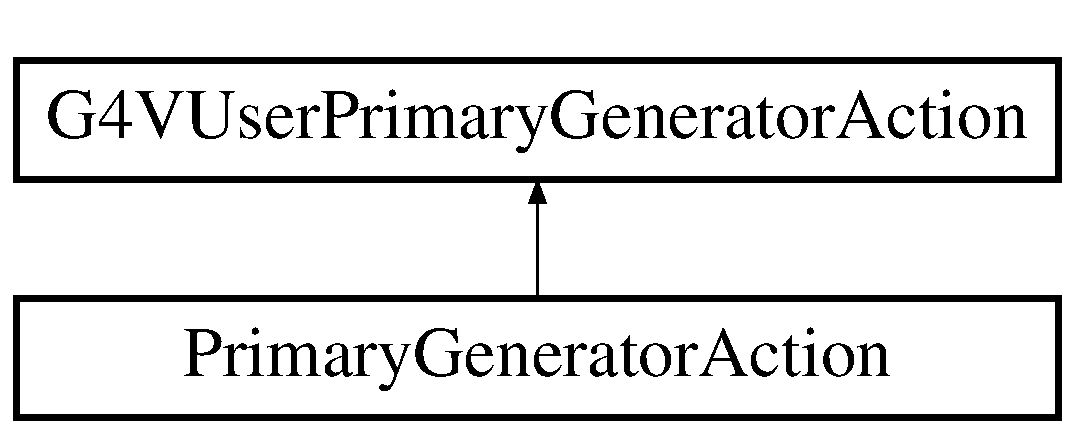
\includegraphics[height=2.000000cm]{class_primary_generator_action}
\end{center}
\end{figure}
\subsection*{Public Member Functions}
\begin{DoxyCompactItemize}
\item 
\hyperlink{class_primary_generator_action_a4bbef83d397d84b434541f8720bf747d}{Primary\-Generator\-Action} ()
\item 
\hyperlink{class_primary_generator_action_ad236fbc210171b9178446778b6bdfb40}{$\sim$\-Primary\-Generator\-Action} ()
\item 
void \hyperlink{class_primary_generator_action_a67d83efdbb2b6e6f97a001dc921ea003}{Generate\-Primaries} (G4\-Event $\ast$an\-Event)
\end{DoxyCompactItemize}


\subsection{Detailed Description}


Definition at line 14 of file Primary\-Generator\-Action.\-hh.



\subsection{Constructor \& Destructor Documentation}
\hypertarget{class_primary_generator_action_a4bbef83d397d84b434541f8720bf747d}{\index{Primary\-Generator\-Action@{Primary\-Generator\-Action}!Primary\-Generator\-Action@{Primary\-Generator\-Action}}
\index{Primary\-Generator\-Action@{Primary\-Generator\-Action}!PrimaryGeneratorAction@{Primary\-Generator\-Action}}
\subsubsection[{Primary\-Generator\-Action}]{\setlength{\rightskip}{0pt plus 5cm}Primary\-Generator\-Action\-::\-Primary\-Generator\-Action (
\begin{DoxyParamCaption}
{}
\end{DoxyParamCaption}
)}}\label{class_primary_generator_action_a4bbef83d397d84b434541f8720bf747d}


Definition at line 14 of file Primary\-Generator\-Action.\-cc.

\hypertarget{class_primary_generator_action_ad236fbc210171b9178446778b6bdfb40}{\index{Primary\-Generator\-Action@{Primary\-Generator\-Action}!$\sim$\-Primary\-Generator\-Action@{$\sim$\-Primary\-Generator\-Action}}
\index{$\sim$\-Primary\-Generator\-Action@{$\sim$\-Primary\-Generator\-Action}!PrimaryGeneratorAction@{Primary\-Generator\-Action}}
\subsubsection[{$\sim$\-Primary\-Generator\-Action}]{\setlength{\rightskip}{0pt plus 5cm}Primary\-Generator\-Action\-::$\sim$\-Primary\-Generator\-Action (
\begin{DoxyParamCaption}
{}
\end{DoxyParamCaption}
)}}\label{class_primary_generator_action_ad236fbc210171b9178446778b6bdfb40}


Definition at line 27 of file Primary\-Generator\-Action.\-cc.



\subsection{Member Function Documentation}
\hypertarget{class_primary_generator_action_a67d83efdbb2b6e6f97a001dc921ea003}{\index{Primary\-Generator\-Action@{Primary\-Generator\-Action}!Generate\-Primaries@{Generate\-Primaries}}
\index{Generate\-Primaries@{Generate\-Primaries}!PrimaryGeneratorAction@{Primary\-Generator\-Action}}
\subsubsection[{Generate\-Primaries}]{\setlength{\rightskip}{0pt plus 5cm}void Primary\-Generator\-Action\-::\-Generate\-Primaries (
\begin{DoxyParamCaption}
\item[{G4\-Event $\ast$}]{an\-Event}
\end{DoxyParamCaption}
)}}\label{class_primary_generator_action_a67d83efdbb2b6e6f97a001dc921ea003}


Definition at line 32 of file Primary\-Generator\-Action.\-cc.



The documentation for this class was generated from the following files\-:\begin{DoxyCompactItemize}
\item 
/\-Users/sandro/g4work/\-Geant4\-Master\-Dissertation\-Simulation/include/\hyperlink{_primary_generator_action_8hh}{Primary\-Generator\-Action.\-hh}\item 
/\-Users/sandro/g4work/\-Geant4\-Master\-Dissertation\-Simulation/src/\hyperlink{_primary_generator_action_8cc}{Primary\-Generator\-Action.\-cc}\end{DoxyCompactItemize}

\hypertarget{class_run}{\section{Run Class Reference}
\label{class_run}\index{Run@{Run}}
}


{\ttfamily \#include $<$Run.\-hh$>$}

Inheritance diagram for Run\-:\begin{figure}[H]
\begin{center}
\leavevmode
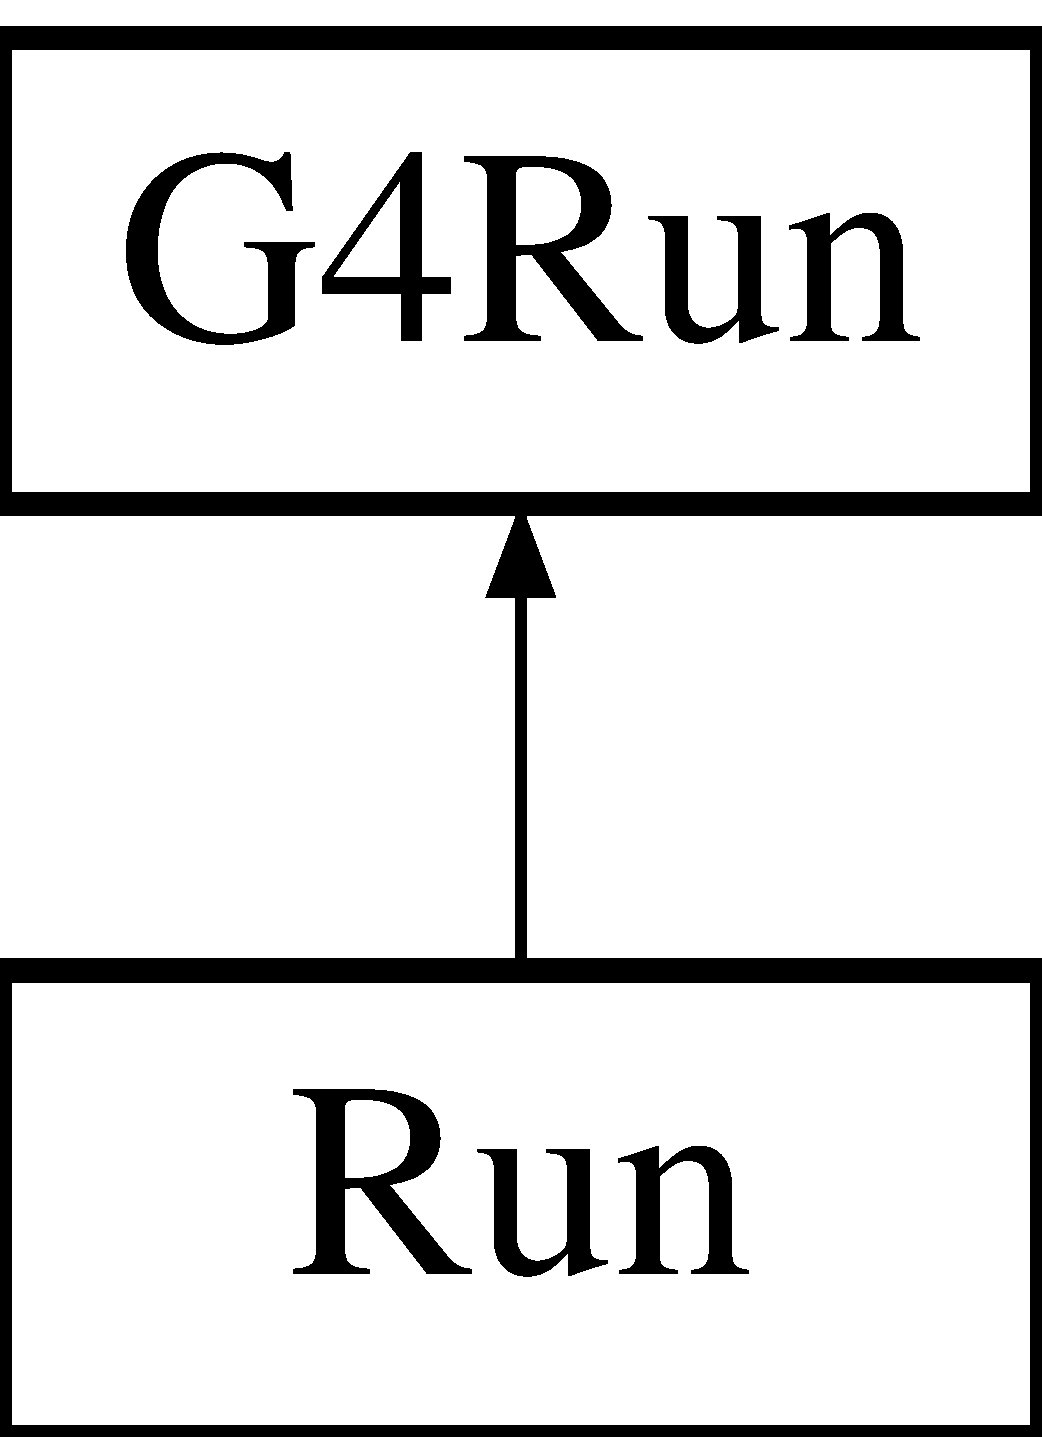
\includegraphics[height=2.000000cm]{class_run}
\end{center}
\end{figure}
\subsection*{Public Member Functions}
\begin{DoxyCompactItemize}
\item 
\hyperlink{class_run_ad9511732117430d7fcdc0c11796f0ef6}{Run} ()
\item 
virtual \hyperlink{class_run_a7fa0ac1770a5067113aaa1928be3d742}{$\sim$\-Run} ()
\item 
virtual void \hyperlink{class_run_a8476edf182546b547d1be728b477e379}{Record\-Event} (const G4\-Event $\ast$)
\item 
G4double \hyperlink{class_run_a7e6a4d99e20df653d53ff8e88f3c3d63}{Get\-Total\-Energy\-Deposited} () const 
\end{DoxyCompactItemize}


\subsection{Detailed Description}


Definition at line 12 of file Run.\-hh.



\subsection{Constructor \& Destructor Documentation}
\hypertarget{class_run_ad9511732117430d7fcdc0c11796f0ef6}{\index{Run@{Run}!Run@{Run}}
\index{Run@{Run}!Run@{Run}}
\subsubsection[{Run}]{\setlength{\rightskip}{0pt plus 5cm}Run\-::\-Run (
\begin{DoxyParamCaption}
{}
\end{DoxyParamCaption}
)}}\label{class_run_ad9511732117430d7fcdc0c11796f0ef6}
\begin{DoxyAuthor}{Author}
Sandro Boschetti, August 28, 2012
\end{DoxyAuthor}
This class is based in the Geant4's Example 07 class. 

Definition at line 14 of file Run.\-cc.

\hypertarget{class_run_a7fa0ac1770a5067113aaa1928be3d742}{\index{Run@{Run}!$\sim$\-Run@{$\sim$\-Run}}
\index{$\sim$\-Run@{$\sim$\-Run}!Run@{Run}}
\subsubsection[{$\sim$\-Run}]{\setlength{\rightskip}{0pt plus 5cm}Run\-::$\sim$\-Run (
\begin{DoxyParamCaption}
{}
\end{DoxyParamCaption}
)\hspace{0.3cm}{\ttfamily [virtual]}}}\label{class_run_a7fa0ac1770a5067113aaa1928be3d742}


Definition at line 21 of file Run.\-cc.



\subsection{Member Function Documentation}
\hypertarget{class_run_a7e6a4d99e20df653d53ff8e88f3c3d63}{\index{Run@{Run}!Get\-Total\-Energy\-Deposited@{Get\-Total\-Energy\-Deposited}}
\index{Get\-Total\-Energy\-Deposited@{Get\-Total\-Energy\-Deposited}!Run@{Run}}
\subsubsection[{Get\-Total\-Energy\-Deposited}]{\setlength{\rightskip}{0pt plus 5cm}G4double Run\-::\-Get\-Total\-Energy\-Deposited (
\begin{DoxyParamCaption}
{}
\end{DoxyParamCaption}
) const\hspace{0.3cm}{\ttfamily [inline]}}}\label{class_run_a7e6a4d99e20df653d53ff8e88f3c3d63}


Definition at line 21 of file Run.\-hh.

\hypertarget{class_run_a8476edf182546b547d1be728b477e379}{\index{Run@{Run}!Record\-Event@{Record\-Event}}
\index{Record\-Event@{Record\-Event}!Run@{Run}}
\subsubsection[{Record\-Event}]{\setlength{\rightskip}{0pt plus 5cm}void Run\-::\-Record\-Event (
\begin{DoxyParamCaption}
\item[{const G4\-Event $\ast$}]{evt}
\end{DoxyParamCaption}
)\hspace{0.3cm}{\ttfamily [virtual]}}}\label{class_run_a8476edf182546b547d1be728b477e379}


Definition at line 24 of file Run.\-cc.



The documentation for this class was generated from the following files\-:\begin{DoxyCompactItemize}
\item 
\hyperlink{_run_8hh}{Run.\-hh}\item 
\hyperlink{_run_8cc}{Run.\-cc}\end{DoxyCompactItemize}

\hypertarget{class_run_action}{\section{Run\-Action Class Reference}
\label{class_run_action}\index{Run\-Action@{Run\-Action}}
}


{\ttfamily \#include $<$Run\-Action.\-hh$>$}

Inheritance diagram for Run\-Action\-:\begin{figure}[H]
\begin{center}
\leavevmode
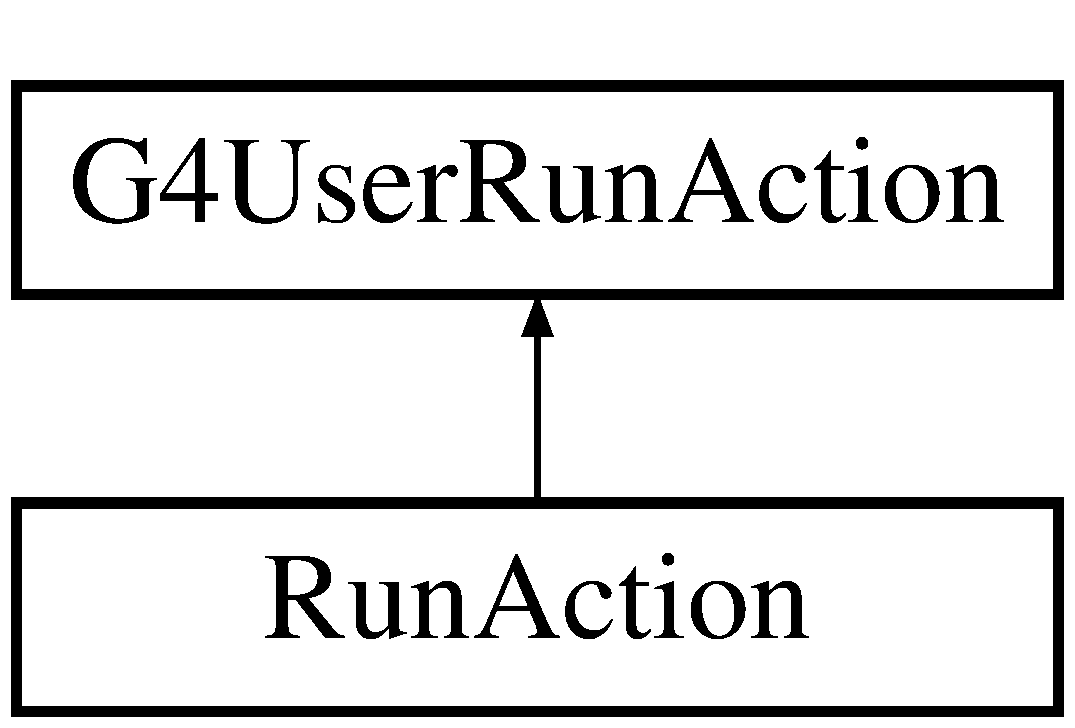
\includegraphics[height=2.000000cm]{class_run_action}
\end{center}
\end{figure}
\subsection*{Public Member Functions}
\begin{DoxyCompactItemize}
\item 
\hyperlink{class_run_action_a535a70dd2811b2212753372dcb5a2f50}{Run\-Action} ()
\item 
\hyperlink{class_run_action_a6c584eb414c62a6238d5ea9a55601e1c}{$\sim$\-Run\-Action} ()
\item 
G4\-Run $\ast$ \hyperlink{class_run_action_ae4b3ac26ec0dbde4b1ebfc4f499c3b7c}{Generate\-Run} ()
\begin{DoxyCompactList}\small\item\em This is the connection between \hyperlink{class_run_action}{Run\-Action} and \hyperlink{class_run}{Run} classes. \end{DoxyCompactList}\item 
virtual void \hyperlink{class_run_action_a14b3433a6875194c4adfe1c222884f0d}{Begin\-Of\-Run\-Action} (const G4\-Run $\ast$)
\item 
virtual void \hyperlink{class_run_action_a49e3c5db63358317c3babca100163bd9}{End\-Of\-Run\-Action} (const G4\-Run $\ast$)
\end{DoxyCompactItemize}


\subsection{Detailed Description}


Definition at line 10 of file Run\-Action.\-hh.



\subsection{Constructor \& Destructor Documentation}
\hypertarget{class_run_action_a535a70dd2811b2212753372dcb5a2f50}{\index{Run\-Action@{Run\-Action}!Run\-Action@{Run\-Action}}
\index{Run\-Action@{Run\-Action}!RunAction@{Run\-Action}}
\subsubsection[{Run\-Action}]{\setlength{\rightskip}{0pt plus 5cm}Run\-Action\-::\-Run\-Action (
\begin{DoxyParamCaption}
{}
\end{DoxyParamCaption}
)}}\label{class_run_action_a535a70dd2811b2212753372dcb5a2f50}
\begin{DoxyAuthor}{Author}
Sandro Boschetti, August 28, 2012
\end{DoxyAuthor}
This class is based in the Geant4's Example 07 class. 

Definition at line 22 of file src/\-Run\-Action.\-cc.

\hypertarget{class_run_action_a6c584eb414c62a6238d5ea9a55601e1c}{\index{Run\-Action@{Run\-Action}!$\sim$\-Run\-Action@{$\sim$\-Run\-Action}}
\index{$\sim$\-Run\-Action@{$\sim$\-Run\-Action}!RunAction@{Run\-Action}}
\subsubsection[{$\sim$\-Run\-Action}]{\setlength{\rightskip}{0pt plus 5cm}Run\-Action\-::$\sim$\-Run\-Action (
\begin{DoxyParamCaption}
{}
\end{DoxyParamCaption}
)}}\label{class_run_action_a6c584eb414c62a6238d5ea9a55601e1c}


Definition at line 24 of file src/\-Run\-Action.\-cc.



\subsection{Member Function Documentation}
\hypertarget{class_run_action_a14b3433a6875194c4adfe1c222884f0d}{\index{Run\-Action@{Run\-Action}!Begin\-Of\-Run\-Action@{Begin\-Of\-Run\-Action}}
\index{Begin\-Of\-Run\-Action@{Begin\-Of\-Run\-Action}!RunAction@{Run\-Action}}
\subsubsection[{Begin\-Of\-Run\-Action}]{\setlength{\rightskip}{0pt plus 5cm}void Run\-Action\-::\-Begin\-Of\-Run\-Action (
\begin{DoxyParamCaption}
\item[{const G4\-Run $\ast$}]{}
\end{DoxyParamCaption}
)\hspace{0.3cm}{\ttfamily [virtual]}}}\label{class_run_action_a14b3433a6875194c4adfe1c222884f0d}


Definition at line 33 of file src/\-Run\-Action.\-cc.

\hypertarget{class_run_action_a49e3c5db63358317c3babca100163bd9}{\index{Run\-Action@{Run\-Action}!End\-Of\-Run\-Action@{End\-Of\-Run\-Action}}
\index{End\-Of\-Run\-Action@{End\-Of\-Run\-Action}!RunAction@{Run\-Action}}
\subsubsection[{End\-Of\-Run\-Action}]{\setlength{\rightskip}{0pt plus 5cm}void Run\-Action\-::\-End\-Of\-Run\-Action (
\begin{DoxyParamCaption}
\item[{const G4\-Run $\ast$}]{a\-Run}
\end{DoxyParamCaption}
)\hspace{0.3cm}{\ttfamily [virtual]}}}\label{class_run_action_a49e3c5db63358317c3babca100163bd9}


Definition at line 37 of file src/\-Run\-Action.\-cc.

\hypertarget{class_run_action_ae4b3ac26ec0dbde4b1ebfc4f499c3b7c}{\index{Run\-Action@{Run\-Action}!Generate\-Run@{Generate\-Run}}
\index{Generate\-Run@{Generate\-Run}!RunAction@{Run\-Action}}
\subsubsection[{Generate\-Run}]{\setlength{\rightskip}{0pt plus 5cm}G4\-Run $\ast$ Run\-Action\-::\-Generate\-Run (
\begin{DoxyParamCaption}
{}
\end{DoxyParamCaption}
)}}\label{class_run_action_ae4b3ac26ec0dbde4b1ebfc4f499c3b7c}


This is the connection between \hyperlink{class_run_action}{Run\-Action} and \hyperlink{class_run}{Run} classes. 

This is te connection between \hyperlink{class_run_action}{Run\-Action} and \hyperlink{class_run}{Run} classes. 

Definition at line 29 of file src/\-Run\-Action.\-cc.



The documentation for this class was generated from the following files\-:\begin{DoxyCompactItemize}
\item 
\hyperlink{_run_action_8hh}{Run\-Action.\-hh}\item 
\hyperlink{src_2_run_action_8cc}{src/\-Run\-Action.\-cc}\item 
\hyperlink{stuff_2_run_action_8cc}{stuff/\-Run\-Action.\-cc}\end{DoxyCompactItemize}

\hypertarget{class_teste}{\section{Teste Class Reference}
\label{class_teste}\index{Teste@{Teste}}
}


{\ttfamily \#include $<$Teste.\-hh$>$}

\subsection*{Public Member Functions}
\begin{DoxyCompactItemize}
\item 
\hyperlink{class_teste_ae6316d96999cf9040acf510edf597e51}{Teste} ()
\item 
virtual \hyperlink{class_teste_a0898d59c63f1aead610427a0696c24ec}{$\sim$\-Teste} ()
\end{DoxyCompactItemize}
\subsection*{Static Public Attributes}
\begin{DoxyCompactItemize}
\item 
static int \hyperlink{class_teste_a12621c33e0d80377802310ef95220f00}{teste} = 0
\end{DoxyCompactItemize}


\subsection{Detailed Description}


Definition at line 11 of file Teste.\-hh.



\subsection{Constructor \& Destructor Documentation}
\hypertarget{class_teste_ae6316d96999cf9040acf510edf597e51}{\index{Teste@{Teste}!Teste@{Teste}}
\index{Teste@{Teste}!Teste@{Teste}}
\subsubsection[{Teste}]{\setlength{\rightskip}{0pt plus 5cm}Teste\-::\-Teste (
\begin{DoxyParamCaption}
{}
\end{DoxyParamCaption}
)}}\label{class_teste_ae6316d96999cf9040acf510edf597e51}


Definition at line 10 of file Teste.\-cc.

\hypertarget{class_teste_a0898d59c63f1aead610427a0696c24ec}{\index{Teste@{Teste}!$\sim$\-Teste@{$\sim$\-Teste}}
\index{$\sim$\-Teste@{$\sim$\-Teste}!Teste@{Teste}}
\subsubsection[{$\sim$\-Teste}]{\setlength{\rightskip}{0pt plus 5cm}Teste\-::$\sim$\-Teste (
\begin{DoxyParamCaption}
{}
\end{DoxyParamCaption}
)\hspace{0.3cm}{\ttfamily [virtual]}}}\label{class_teste_a0898d59c63f1aead610427a0696c24ec}


Definition at line 14 of file Teste.\-cc.



\subsection{Member Data Documentation}
\hypertarget{class_teste_a12621c33e0d80377802310ef95220f00}{\index{Teste@{Teste}!teste@{teste}}
\index{teste@{teste}!Teste@{Teste}}
\subsubsection[{teste}]{\setlength{\rightskip}{0pt plus 5cm}int Teste\-::teste = 0\hspace{0.3cm}{\ttfamily [static]}}}\label{class_teste_a12621c33e0d80377802310ef95220f00}


Definition at line 15 of file Teste.\-hh.



The documentation for this class was generated from the following files\-:\begin{DoxyCompactItemize}
\item 
\hyperlink{_teste_8hh}{Teste.\-hh}\item 
\hyperlink{_teste_8cc}{Teste.\-cc}\end{DoxyCompactItemize}

\hypertarget{class_teste_detector_construction}{\section{Teste\-Detector\-Construction Class Reference}
\label{class_teste_detector_construction}\index{Teste\-Detector\-Construction@{Teste\-Detector\-Construction}}
}


{\ttfamily \#include $<$Teste\-Detector\-Construction.\-hh$>$}

Inheritance diagram for Teste\-Detector\-Construction\-:\begin{figure}[H]
\begin{center}
\leavevmode
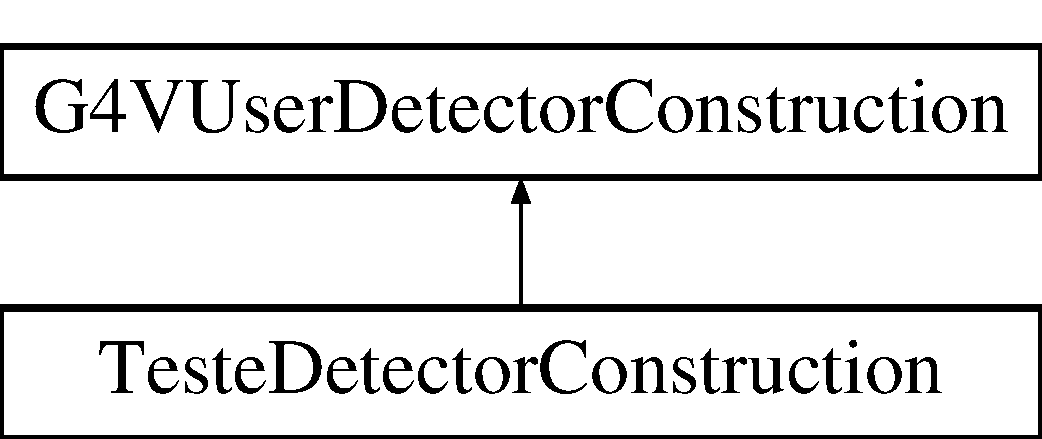
\includegraphics[height=2.000000cm]{class_teste_detector_construction}
\end{center}
\end{figure}
\subsection*{Public Member Functions}
\begin{DoxyCompactItemize}
\item 
\hyperlink{class_teste_detector_construction_acbda0bce688e1d85e613f9ce8f63c921}{Teste\-Detector\-Construction} ()
\item 
\hyperlink{class_teste_detector_construction_a54bb831b6727d9208703ed9a8408c2ea}{$\sim$\-Teste\-Detector\-Construction} ()
\item 
G4\-V\-Physical\-Volume $\ast$ \hyperlink{class_teste_detector_construction_aa3d65155773b1d8c1b65f2c91c7cac47}{Construct} ()
\end{DoxyCompactItemize}


\subsection{Detailed Description}


Definition at line 14 of file Teste\-Detector\-Construction.\-hh.



\subsection{Constructor \& Destructor Documentation}
\hypertarget{class_teste_detector_construction_acbda0bce688e1d85e613f9ce8f63c921}{\index{Teste\-Detector\-Construction@{Teste\-Detector\-Construction}!Teste\-Detector\-Construction@{Teste\-Detector\-Construction}}
\index{Teste\-Detector\-Construction@{Teste\-Detector\-Construction}!TesteDetectorConstruction@{Teste\-Detector\-Construction}}
\subsubsection[{Teste\-Detector\-Construction}]{\setlength{\rightskip}{0pt plus 5cm}Teste\-Detector\-Construction\-::\-Teste\-Detector\-Construction (
\begin{DoxyParamCaption}
{}
\end{DoxyParamCaption}
)}}\label{class_teste_detector_construction_acbda0bce688e1d85e613f9ce8f63c921}


Definition at line 16 of file Teste\-Detector\-Construction.\-cc.

\hypertarget{class_teste_detector_construction_a54bb831b6727d9208703ed9a8408c2ea}{\index{Teste\-Detector\-Construction@{Teste\-Detector\-Construction}!$\sim$\-Teste\-Detector\-Construction@{$\sim$\-Teste\-Detector\-Construction}}
\index{$\sim$\-Teste\-Detector\-Construction@{$\sim$\-Teste\-Detector\-Construction}!TesteDetectorConstruction@{Teste\-Detector\-Construction}}
\subsubsection[{$\sim$\-Teste\-Detector\-Construction}]{\setlength{\rightskip}{0pt plus 5cm}Teste\-Detector\-Construction\-::$\sim$\-Teste\-Detector\-Construction (
\begin{DoxyParamCaption}
{}
\end{DoxyParamCaption}
)}}\label{class_teste_detector_construction_a54bb831b6727d9208703ed9a8408c2ea}


Definition at line 23 of file Teste\-Detector\-Construction.\-cc.



\subsection{Member Function Documentation}
\hypertarget{class_teste_detector_construction_aa3d65155773b1d8c1b65f2c91c7cac47}{\index{Teste\-Detector\-Construction@{Teste\-Detector\-Construction}!Construct@{Construct}}
\index{Construct@{Construct}!TesteDetectorConstruction@{Teste\-Detector\-Construction}}
\subsubsection[{Construct}]{\setlength{\rightskip}{0pt plus 5cm}G4\-V\-Physical\-Volume $\ast$ Teste\-Detector\-Construction\-::\-Construct (
\begin{DoxyParamCaption}
{}
\end{DoxyParamCaption}
)}}\label{class_teste_detector_construction_aa3d65155773b1d8c1b65f2c91c7cac47}


Definition at line 27 of file Teste\-Detector\-Construction.\-cc.



The documentation for this class was generated from the following files\-:\begin{DoxyCompactItemize}
\item 
\hyperlink{_teste_detector_construction_8hh}{Teste\-Detector\-Construction.\-hh}\item 
\hyperlink{_teste_detector_construction_8cc}{Teste\-Detector\-Construction.\-cc}\end{DoxyCompactItemize}

\hypertarget{class_teste_physics_list}{\section{Teste\-Physics\-List Class Reference}
\label{class_teste_physics_list}\index{Teste\-Physics\-List@{Teste\-Physics\-List}}
}


{\ttfamily \#include $<$Teste\-Physics\-List.\-hh$>$}

Inheritance diagram for Teste\-Physics\-List\-:\begin{figure}[H]
\begin{center}
\leavevmode
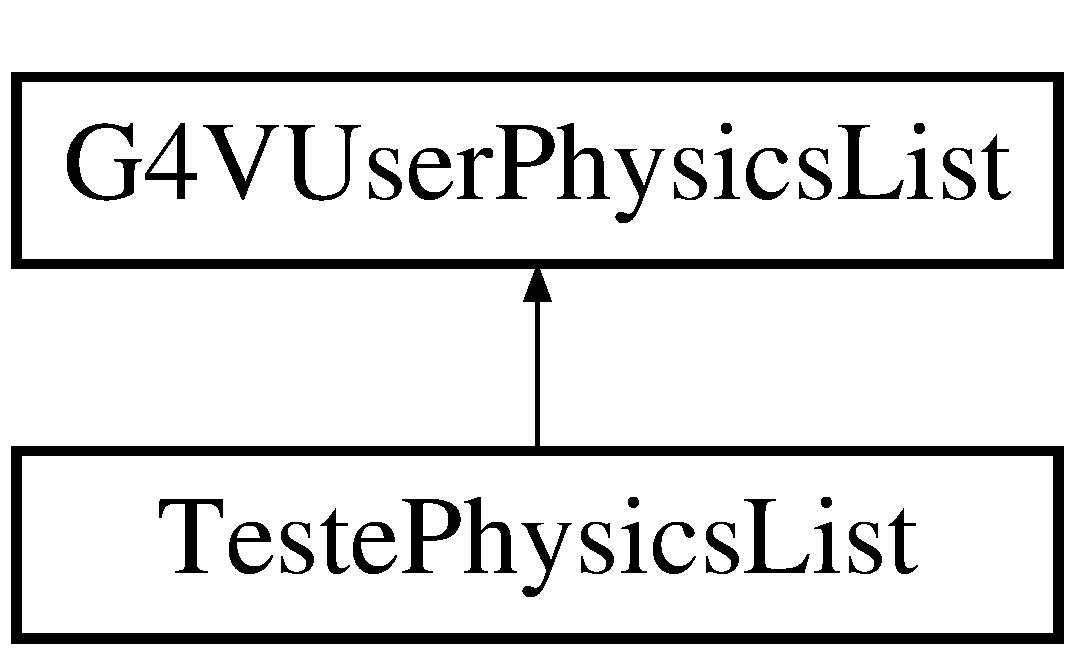
\includegraphics[height=2.000000cm]{class_teste_physics_list}
\end{center}
\end{figure}
\subsection*{Public Member Functions}
\begin{DoxyCompactItemize}
\item 
\hyperlink{class_teste_physics_list_a80905ad5c634c9672b6bec654f572562}{Teste\-Physics\-List} ()
\item 
\hyperlink{class_teste_physics_list_a47937c7e6c6a8d259e23735ca6e148ad}{$\sim$\-Teste\-Physics\-List} ()
\end{DoxyCompactItemize}
\subsection*{Protected Member Functions}
\begin{DoxyCompactItemize}
\item 
void \hyperlink{class_teste_physics_list_a529073a7fd79b97abff758b3f600a0dd}{Construct\-Particle} ()
\item 
void \hyperlink{class_teste_physics_list_a43e995eecc08bf708ed6f699fb095eb8}{Construct\-Process} ()
\item 
void \hyperlink{class_teste_physics_list_a79bcd77a2c7cd8e7469636107657c666}{Set\-Cuts} ()
\end{DoxyCompactItemize}


\subsection{Detailed Description}


Definition at line 13 of file Teste\-Physics\-List.\-hh.



\subsection{Constructor \& Destructor Documentation}
\hypertarget{class_teste_physics_list_a80905ad5c634c9672b6bec654f572562}{\index{Teste\-Physics\-List@{Teste\-Physics\-List}!Teste\-Physics\-List@{Teste\-Physics\-List}}
\index{Teste\-Physics\-List@{Teste\-Physics\-List}!TestePhysicsList@{Teste\-Physics\-List}}
\subsubsection[{Teste\-Physics\-List}]{\setlength{\rightskip}{0pt plus 5cm}Teste\-Physics\-List\-::\-Teste\-Physics\-List (
\begin{DoxyParamCaption}
{}
\end{DoxyParamCaption}
)}}\label{class_teste_physics_list_a80905ad5c634c9672b6bec654f572562}


Definition at line 11 of file Teste\-Physics\-List.\-cc.

\hypertarget{class_teste_physics_list_a47937c7e6c6a8d259e23735ca6e148ad}{\index{Teste\-Physics\-List@{Teste\-Physics\-List}!$\sim$\-Teste\-Physics\-List@{$\sim$\-Teste\-Physics\-List}}
\index{$\sim$\-Teste\-Physics\-List@{$\sim$\-Teste\-Physics\-List}!TestePhysicsList@{Teste\-Physics\-List}}
\subsubsection[{$\sim$\-Teste\-Physics\-List}]{\setlength{\rightskip}{0pt plus 5cm}Teste\-Physics\-List\-::$\sim$\-Teste\-Physics\-List (
\begin{DoxyParamCaption}
{}
\end{DoxyParamCaption}
)}}\label{class_teste_physics_list_a47937c7e6c6a8d259e23735ca6e148ad}


Definition at line 14 of file Teste\-Physics\-List.\-cc.



\subsection{Member Function Documentation}
\hypertarget{class_teste_physics_list_a529073a7fd79b97abff758b3f600a0dd}{\index{Teste\-Physics\-List@{Teste\-Physics\-List}!Construct\-Particle@{Construct\-Particle}}
\index{Construct\-Particle@{Construct\-Particle}!TestePhysicsList@{Teste\-Physics\-List}}
\subsubsection[{Construct\-Particle}]{\setlength{\rightskip}{0pt plus 5cm}void Teste\-Physics\-List\-::\-Construct\-Particle (
\begin{DoxyParamCaption}
{}
\end{DoxyParamCaption}
)\hspace{0.3cm}{\ttfamily [protected]}}}\label{class_teste_physics_list_a529073a7fd79b97abff758b3f600a0dd}


Definition at line 17 of file Teste\-Physics\-List.\-cc.

\hypertarget{class_teste_physics_list_a43e995eecc08bf708ed6f699fb095eb8}{\index{Teste\-Physics\-List@{Teste\-Physics\-List}!Construct\-Process@{Construct\-Process}}
\index{Construct\-Process@{Construct\-Process}!TestePhysicsList@{Teste\-Physics\-List}}
\subsubsection[{Construct\-Process}]{\setlength{\rightskip}{0pt plus 5cm}void Teste\-Physics\-List\-::\-Construct\-Process (
\begin{DoxyParamCaption}
{}
\end{DoxyParamCaption}
)\hspace{0.3cm}{\ttfamily [protected]}}}\label{class_teste_physics_list_a43e995eecc08bf708ed6f699fb095eb8}


Definition at line 27 of file Teste\-Physics\-List.\-cc.

\hypertarget{class_teste_physics_list_a79bcd77a2c7cd8e7469636107657c666}{\index{Teste\-Physics\-List@{Teste\-Physics\-List}!Set\-Cuts@{Set\-Cuts}}
\index{Set\-Cuts@{Set\-Cuts}!TestePhysicsList@{Teste\-Physics\-List}}
\subsubsection[{Set\-Cuts}]{\setlength{\rightskip}{0pt plus 5cm}void Teste\-Physics\-List\-::\-Set\-Cuts (
\begin{DoxyParamCaption}
{}
\end{DoxyParamCaption}
)\hspace{0.3cm}{\ttfamily [protected]}}}\label{class_teste_physics_list_a79bcd77a2c7cd8e7469636107657c666}


Definition at line 34 of file Teste\-Physics\-List.\-cc.



The documentation for this class was generated from the following files\-:\begin{DoxyCompactItemize}
\item 
\hyperlink{_teste_physics_list_8hh}{Teste\-Physics\-List.\-hh}\item 
\hyperlink{_teste_physics_list_8cc}{Teste\-Physics\-List.\-cc}\end{DoxyCompactItemize}

\hypertarget{class_teste_primary_generator_action}{\section{Teste\-Primary\-Generator\-Action Class Reference}
\label{class_teste_primary_generator_action}\index{Teste\-Primary\-Generator\-Action@{Teste\-Primary\-Generator\-Action}}
}


{\ttfamily \#include $<$Teste\-Primary\-Generator\-Action.\-hh$>$}

Inheritance diagram for Teste\-Primary\-Generator\-Action\-:\begin{figure}[H]
\begin{center}
\leavevmode
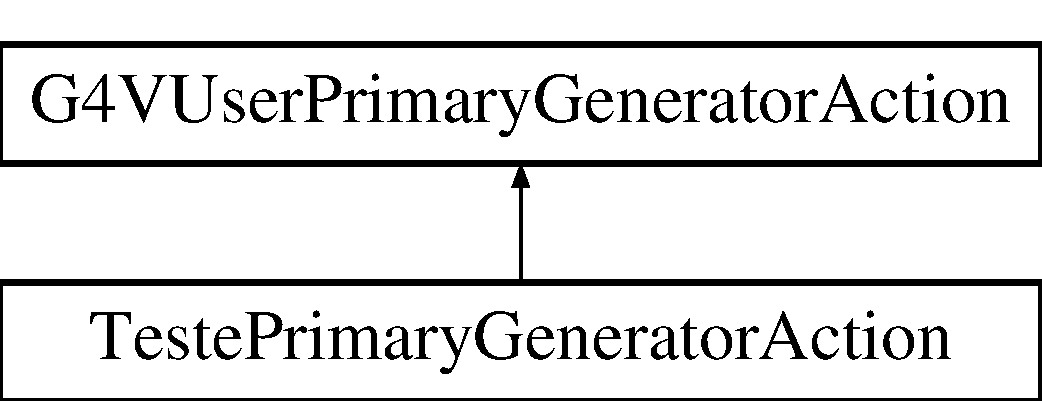
\includegraphics[height=2.000000cm]{class_teste_primary_generator_action}
\end{center}
\end{figure}
\subsection*{Public Member Functions}
\begin{DoxyCompactItemize}
\item 
\hyperlink{class_teste_primary_generator_action_a8316c9aa1d5a826a990328174f45acbc}{Teste\-Primary\-Generator\-Action} ()
\item 
\hyperlink{class_teste_primary_generator_action_a41ad8aaf19501a10e8196b4f03e964c8}{$\sim$\-Teste\-Primary\-Generator\-Action} ()
\item 
void \hyperlink{class_teste_primary_generator_action_a1053cfce172f6d45dd8d5927ac9db3eb}{Generate\-Primaries} (G4\-Event $\ast$an\-Event)
\end{DoxyCompactItemize}


\subsection{Detailed Description}


Definition at line 14 of file Teste\-Primary\-Generator\-Action.\-hh.



\subsection{Constructor \& Destructor Documentation}
\hypertarget{class_teste_primary_generator_action_a8316c9aa1d5a826a990328174f45acbc}{\index{Teste\-Primary\-Generator\-Action@{Teste\-Primary\-Generator\-Action}!Teste\-Primary\-Generator\-Action@{Teste\-Primary\-Generator\-Action}}
\index{Teste\-Primary\-Generator\-Action@{Teste\-Primary\-Generator\-Action}!TestePrimaryGeneratorAction@{Teste\-Primary\-Generator\-Action}}
\subsubsection[{Teste\-Primary\-Generator\-Action}]{\setlength{\rightskip}{0pt plus 5cm}Teste\-Primary\-Generator\-Action\-::\-Teste\-Primary\-Generator\-Action (
\begin{DoxyParamCaption}
{}
\end{DoxyParamCaption}
)}}\label{class_teste_primary_generator_action_a8316c9aa1d5a826a990328174f45acbc}


Definition at line 14 of file Teste\-Primary\-Generator\-Action.\-cc.

\hypertarget{class_teste_primary_generator_action_a41ad8aaf19501a10e8196b4f03e964c8}{\index{Teste\-Primary\-Generator\-Action@{Teste\-Primary\-Generator\-Action}!$\sim$\-Teste\-Primary\-Generator\-Action@{$\sim$\-Teste\-Primary\-Generator\-Action}}
\index{$\sim$\-Teste\-Primary\-Generator\-Action@{$\sim$\-Teste\-Primary\-Generator\-Action}!TestePrimaryGeneratorAction@{Teste\-Primary\-Generator\-Action}}
\subsubsection[{$\sim$\-Teste\-Primary\-Generator\-Action}]{\setlength{\rightskip}{0pt plus 5cm}Teste\-Primary\-Generator\-Action\-::$\sim$\-Teste\-Primary\-Generator\-Action (
\begin{DoxyParamCaption}
{}
\end{DoxyParamCaption}
)}}\label{class_teste_primary_generator_action_a41ad8aaf19501a10e8196b4f03e964c8}


Definition at line 26 of file Teste\-Primary\-Generator\-Action.\-cc.



\subsection{Member Function Documentation}
\hypertarget{class_teste_primary_generator_action_a1053cfce172f6d45dd8d5927ac9db3eb}{\index{Teste\-Primary\-Generator\-Action@{Teste\-Primary\-Generator\-Action}!Generate\-Primaries@{Generate\-Primaries}}
\index{Generate\-Primaries@{Generate\-Primaries}!TestePrimaryGeneratorAction@{Teste\-Primary\-Generator\-Action}}
\subsubsection[{Generate\-Primaries}]{\setlength{\rightskip}{0pt plus 5cm}void Teste\-Primary\-Generator\-Action\-::\-Generate\-Primaries (
\begin{DoxyParamCaption}
\item[{G4\-Event $\ast$}]{an\-Event}
\end{DoxyParamCaption}
)}}\label{class_teste_primary_generator_action_a1053cfce172f6d45dd8d5927ac9db3eb}


Definition at line 31 of file Teste\-Primary\-Generator\-Action.\-cc.



The documentation for this class was generated from the following files\-:\begin{DoxyCompactItemize}
\item 
\hyperlink{_teste_primary_generator_action_8hh}{Teste\-Primary\-Generator\-Action.\-hh}\item 
\hyperlink{_teste_primary_generator_action_8cc}{Teste\-Primary\-Generator\-Action.\-cc}\end{DoxyCompactItemize}

\hypertarget{class_teste_user_run_action}{\section{Teste\-User\-Run\-Action Class Reference}
\label{class_teste_user_run_action}\index{Teste\-User\-Run\-Action@{Teste\-User\-Run\-Action}}
}


{\ttfamily \#include $<$Teste\-User\-Run\-Action.\-hh$>$}

Inheritance diagram for Teste\-User\-Run\-Action\-:\begin{figure}[H]
\begin{center}
\leavevmode
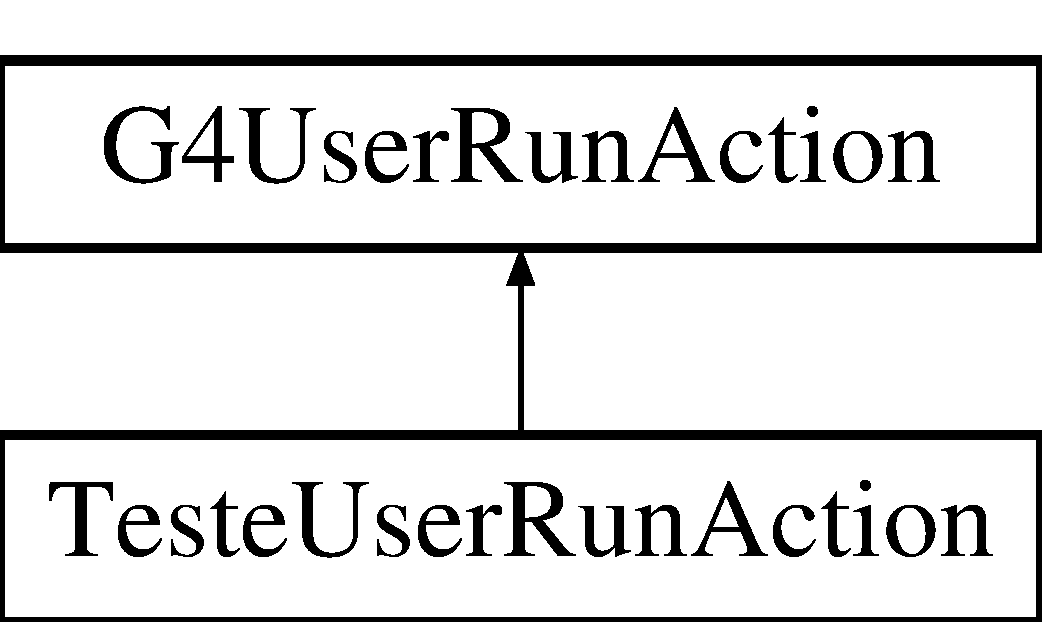
\includegraphics[height=2.000000cm]{class_teste_user_run_action}
\end{center}
\end{figure}
\subsection*{Public Member Functions}
\begin{DoxyCompactItemize}
\item 
\hyperlink{class_teste_user_run_action_a8bde0729eae5ed2ac0030c9d228a7d3d}{Teste\-User\-Run\-Action} ()
\item 
virtual \hyperlink{class_teste_user_run_action_aa09b2e6b369b9b4b073be3ab6cca9d4f}{$\sim$\-Teste\-User\-Run\-Action} ()
\item 
virtual G4\-Run $\ast$ \hyperlink{class_teste_user_run_action_a3a086b2408880a12e757e1381bb5d846}{Generate\-Run} ()
\item 
void \hyperlink{class_teste_user_run_action_abb8bb1bf72adf9b880b680565484582d}{Begin\-Of\-Run\-Action} (const G4\-Run $\ast$)
\item 
void \hyperlink{class_teste_user_run_action_ad638f0a994d5ea37eaa371378d59b522}{End\-Of\-Run\-Action} (const G4\-Run $\ast$)
\end{DoxyCompactItemize}


\subsection{Detailed Description}


Definition at line 10 of file Teste\-User\-Run\-Action.\-hh.



\subsection{Constructor \& Destructor Documentation}
\hypertarget{class_teste_user_run_action_a8bde0729eae5ed2ac0030c9d228a7d3d}{\index{Teste\-User\-Run\-Action@{Teste\-User\-Run\-Action}!Teste\-User\-Run\-Action@{Teste\-User\-Run\-Action}}
\index{Teste\-User\-Run\-Action@{Teste\-User\-Run\-Action}!TesteUserRunAction@{Teste\-User\-Run\-Action}}
\subsubsection[{Teste\-User\-Run\-Action}]{\setlength{\rightskip}{0pt plus 5cm}Teste\-User\-Run\-Action\-::\-Teste\-User\-Run\-Action (
\begin{DoxyParamCaption}
{}
\end{DoxyParamCaption}
)}}\label{class_teste_user_run_action_a8bde0729eae5ed2ac0030c9d228a7d3d}


Definition at line 17 of file Teste\-User\-Run\-Action.\-cc.

\hypertarget{class_teste_user_run_action_aa09b2e6b369b9b4b073be3ab6cca9d4f}{\index{Teste\-User\-Run\-Action@{Teste\-User\-Run\-Action}!$\sim$\-Teste\-User\-Run\-Action@{$\sim$\-Teste\-User\-Run\-Action}}
\index{$\sim$\-Teste\-User\-Run\-Action@{$\sim$\-Teste\-User\-Run\-Action}!TesteUserRunAction@{Teste\-User\-Run\-Action}}
\subsubsection[{$\sim$\-Teste\-User\-Run\-Action}]{\setlength{\rightskip}{0pt plus 5cm}Teste\-User\-Run\-Action\-::$\sim$\-Teste\-User\-Run\-Action (
\begin{DoxyParamCaption}
{}
\end{DoxyParamCaption}
)\hspace{0.3cm}{\ttfamily [virtual]}}}\label{class_teste_user_run_action_aa09b2e6b369b9b4b073be3ab6cca9d4f}


Definition at line 19 of file Teste\-User\-Run\-Action.\-cc.



\subsection{Member Function Documentation}
\hypertarget{class_teste_user_run_action_abb8bb1bf72adf9b880b680565484582d}{\index{Teste\-User\-Run\-Action@{Teste\-User\-Run\-Action}!Begin\-Of\-Run\-Action@{Begin\-Of\-Run\-Action}}
\index{Begin\-Of\-Run\-Action@{Begin\-Of\-Run\-Action}!TesteUserRunAction@{Teste\-User\-Run\-Action}}
\subsubsection[{Begin\-Of\-Run\-Action}]{\setlength{\rightskip}{0pt plus 5cm}void Teste\-User\-Run\-Action\-::\-Begin\-Of\-Run\-Action (
\begin{DoxyParamCaption}
\item[{const G4\-Run $\ast$}]{}
\end{DoxyParamCaption}
)}}\label{class_teste_user_run_action_abb8bb1bf72adf9b880b680565484582d}


Definition at line 21 of file Teste\-User\-Run\-Action.\-cc.

\hypertarget{class_teste_user_run_action_ad638f0a994d5ea37eaa371378d59b522}{\index{Teste\-User\-Run\-Action@{Teste\-User\-Run\-Action}!End\-Of\-Run\-Action@{End\-Of\-Run\-Action}}
\index{End\-Of\-Run\-Action@{End\-Of\-Run\-Action}!TesteUserRunAction@{Teste\-User\-Run\-Action}}
\subsubsection[{End\-Of\-Run\-Action}]{\setlength{\rightskip}{0pt plus 5cm}void Teste\-User\-Run\-Action\-::\-End\-Of\-Run\-Action (
\begin{DoxyParamCaption}
\item[{const G4\-Run $\ast$}]{a\-Run}
\end{DoxyParamCaption}
)}}\label{class_teste_user_run_action_ad638f0a994d5ea37eaa371378d59b522}


Definition at line 29 of file Teste\-User\-Run\-Action.\-cc.

\hypertarget{class_teste_user_run_action_a3a086b2408880a12e757e1381bb5d846}{\index{Teste\-User\-Run\-Action@{Teste\-User\-Run\-Action}!Generate\-Run@{Generate\-Run}}
\index{Generate\-Run@{Generate\-Run}!TesteUserRunAction@{Teste\-User\-Run\-Action}}
\subsubsection[{Generate\-Run}]{\setlength{\rightskip}{0pt plus 5cm}virtual G4\-Run$\ast$ Teste\-User\-Run\-Action\-::\-Generate\-Run (
\begin{DoxyParamCaption}
{}
\end{DoxyParamCaption}
)\hspace{0.3cm}{\ttfamily [virtual]}}}\label{class_teste_user_run_action_a3a086b2408880a12e757e1381bb5d846}


The documentation for this class was generated from the following files\-:\begin{DoxyCompactItemize}
\item 
\hyperlink{_teste_user_run_action_8hh}{Teste\-User\-Run\-Action.\-hh}\item 
\hyperlink{_teste_user_run_action_8cc}{Teste\-User\-Run\-Action.\-cc}\end{DoxyCompactItemize}

\chapter{File Documentation}
\hypertarget{_detector_construction_8cc}{\section{/\-Users/sandro/g4work/\-Geant4\-Master\-Dissertation\-Simulation/src/\-Detector\-Construction.cc File Reference}
\label{_detector_construction_8cc}\index{/\-Users/sandro/g4work/\-Geant4\-Master\-Dissertation\-Simulation/src/\-Detector\-Construction.\-cc@{/\-Users/sandro/g4work/\-Geant4\-Master\-Dissertation\-Simulation/src/\-Detector\-Construction.\-cc}}
}
{\ttfamily \#include \char`\"{}Detector\-Construction.\-hh\char`\"{}}\\*
{\ttfamily \#include \char`\"{}G4\-Material.\-hh\char`\"{}}\\*
{\ttfamily \#include \char`\"{}G4\-Box.\-hh\char`\"{}}\\*
{\ttfamily \#include \char`\"{}G4\-Logical\-Volume.\-hh\char`\"{}}\\*
{\ttfamily \#include \char`\"{}G4\-Three\-Vector.\-hh\char`\"{}}\\*
{\ttfamily \#include \char`\"{}G4\-P\-V\-Placement.\-hh\char`\"{}}\\*
{\ttfamily \#include \char`\"{}G4\-Nist\-Manager.\-hh\char`\"{}}\\*
{\ttfamily \#include \char`\"{}G4\-Vis\-Attributes.\-hh\char`\"{}}\\*

\hypertarget{_detector_construction_8hh}{\section{Detector\-Construction.\-hh File Reference}
\label{_detector_construction_8hh}\index{Detector\-Construction.\-hh@{Detector\-Construction.\-hh}}
}
{\ttfamily \#include \char`\"{}G4\-V\-User\-Detector\-Construction.\-hh\char`\"{}}\\*
\subsection*{Classes}
\begin{DoxyCompactItemize}
\item 
class \hyperlink{class_detector_construction}{Detector\-Construction}
\end{DoxyCompactItemize}

\hypertarget{_geant4_master_dissertation_simulation_8cc}{\section{Geant4\-Master\-Dissertation\-Simulation.\-cc File Reference}
\label{_geant4_master_dissertation_simulation_8cc}\index{Geant4\-Master\-Dissertation\-Simulation.\-cc@{Geant4\-Master\-Dissertation\-Simulation.\-cc}}
}
{\ttfamily \#include $<$ctime$>$}\\*
{\ttfamily \#include \char`\"{}G4\-Run\-Manager.\-hh\char`\"{}}\\*
{\ttfamily \#include \char`\"{}G4\-U\-Imanager.\-hh\char`\"{}}\\*
{\ttfamily \#include \char`\"{}Detector\-Construction.\-hh\char`\"{}}\\*
{\ttfamily \#include \char`\"{}Physics\-List.\-hh\char`\"{}}\\*
{\ttfamily \#include \char`\"{}Primary\-Generator\-Action.\-hh\char`\"{}}\\*
{\ttfamily \#include \char`\"{}Run\-Action.\-hh\char`\"{}}\\*
{\ttfamily \#include $<$pthread.\-h$>$}\\*
\subsection*{Functions}
\begin{DoxyCompactItemize}
\item 
void \hyperlink{_geant4_master_dissertation_simulation_8cc_aa5d649a39a416ee455a5d7c3fcb02f57}{setup\-U\-I\-Programatically} (G4\-U\-Imanager $\ast$U\-I)
\begin{DoxyCompactList}\small\item\em List of classes that must be implemented by the user. \end{DoxyCompactList}\item 
int \hyperlink{_geant4_master_dissertation_simulation_8cc_ab04d39284cce0256e5edcedee1519ece}{main} (G4int argc, char $\ast$$\ast$argv)
\begin{DoxyCompactList}\small\item\em Entry point function for the whole simulation. \end{DoxyCompactList}\end{DoxyCompactItemize}


\subsection{Function Documentation}
\hypertarget{_geant4_master_dissertation_simulation_8cc_ab04d39284cce0256e5edcedee1519ece}{\index{Geant4\-Master\-Dissertation\-Simulation.\-cc@{Geant4\-Master\-Dissertation\-Simulation.\-cc}!main@{main}}
\index{main@{main}!Geant4MasterDissertationSimulation.cc@{Geant4\-Master\-Dissertation\-Simulation.\-cc}}
\subsubsection[{main}]{\setlength{\rightskip}{0pt plus 5cm}int main (
\begin{DoxyParamCaption}
\item[{G4int}]{argc, }
\item[{char $\ast$$\ast$}]{argv}
\end{DoxyParamCaption}
)}}\label{_geant4_master_dissertation_simulation_8cc_ab04d39284cce0256e5edcedee1519ece}


Entry point function for the whole simulation. 

This gets the actual time for simulation duration computation.

Adding user action

This tanslates the physical volume

Definition at line 39 of file Geant4\-Master\-Dissertation\-Simulation.\-cc.

\hypertarget{_geant4_master_dissertation_simulation_8cc_aa5d649a39a416ee455a5d7c3fcb02f57}{\index{Geant4\-Master\-Dissertation\-Simulation.\-cc@{Geant4\-Master\-Dissertation\-Simulation.\-cc}!setup\-U\-I\-Programatically@{setup\-U\-I\-Programatically}}
\index{setup\-U\-I\-Programatically@{setup\-U\-I\-Programatically}!Geant4MasterDissertationSimulation.cc@{Geant4\-Master\-Dissertation\-Simulation.\-cc}}
\subsubsection[{setup\-U\-I\-Programatically}]{\setlength{\rightskip}{0pt plus 5cm}void setup\-U\-I\-Programatically (
\begin{DoxyParamCaption}
\item[{G4\-U\-Imanager $\ast$}]{U\-I}
\end{DoxyParamCaption}
)}}\label{_geant4_master_dissertation_simulation_8cc_aa5d649a39a416ee455a5d7c3fcb02f57}


List of classes that must be implemented by the user. 

This function has been implemented only for a sake of organization.

\begin{DoxyAuthor}{Author}
Sandro Boschetti, August 24, 2012 
\end{DoxyAuthor}
\begin{DoxyVersion}{Version}
0.\-2
\end{DoxyVersion}
This is the main routine, i.\-e., the entry point for the program simulation. It's based on the example N01 from Geant4.\-9.\-3.\-p02. 

Definition at line 178 of file Geant4\-Master\-Dissertation\-Simulation.\-cc.


\hypertarget{_my_material_8cc}{\section{My\-Material.\-cc File Reference}
\label{_my_material_8cc}\index{My\-Material.\-cc@{My\-Material.\-cc}}
}
{\ttfamily \#include \char`\"{}My\-Material.\-hh\char`\"{}}\\*
{\ttfamily \#include \char`\"{}G4\-Material.\-hh\char`\"{}}\\*

\hypertarget{_my_material_8hh}{\section{My\-Material.\-hh File Reference}
\label{_my_material_8hh}\index{My\-Material.\-hh@{My\-Material.\-hh}}
}
\subsection*{Classes}
\begin{DoxyCompactItemize}
\item 
class \hyperlink{class_my_material}{My\-Material}
\end{DoxyCompactItemize}

\hypertarget{_my_random_8cc}{\section{/\-Users/sandro/g4work/\-Geant4\-Master\-Dissertation\-Simulation/src/\-My\-Random.cc File Reference}
\label{_my_random_8cc}\index{/\-Users/sandro/g4work/\-Geant4\-Master\-Dissertation\-Simulation/src/\-My\-Random.\-cc@{/\-Users/sandro/g4work/\-Geant4\-Master\-Dissertation\-Simulation/src/\-My\-Random.\-cc}}
}
{\ttfamily \#include \char`\"{}My\-Random.\-hh\char`\"{}}\\*

\hypertarget{_my_random_8hh}{\section{/\-Users/sandro/g4work/\-Geant4\-Master\-Dissertation\-Simulation/include/\-My\-Random.hh File Reference}
\label{_my_random_8hh}\index{/\-Users/sandro/g4work/\-Geant4\-Master\-Dissertation\-Simulation/include/\-My\-Random.\-hh@{/\-Users/sandro/g4work/\-Geant4\-Master\-Dissertation\-Simulation/include/\-My\-Random.\-hh}}
}
{\ttfamily \#include $<$C\-L\-H\-E\-P/\-Random/\-Randomize.\-h$>$}\\*
{\ttfamily \#include $<$C\-L\-H\-E\-P/\-Random/\-Rand\-Gauss\-Q.\-h$>$}\\*
{\ttfamily \#include $<$C\-L\-H\-E\-P/\-Random/\-Rand\-Gauss\-T.\-h$>$}\\*
{\ttfamily \#include $<$C\-L\-H\-E\-P/\-Random/\-Rand\-Poisson\-Q.\-h$>$}\\*
{\ttfamily \#include $<$C\-L\-H\-E\-P/\-Random/\-Rand\-Poisson\-T.\-h$>$}\\*
{\ttfamily \#include $<$C\-L\-H\-E\-P/\-Random/\-Rand\-Landau.\-h$>$}\\*
{\ttfamily \#include $<$C\-L\-H\-E\-P/\-Random/\-Rand\-Bit.\-h$>$}\\*
\subsection*{Classes}
\begin{DoxyCompactItemize}
\item 
class \hyperlink{class_my_random}{My\-Random}
\end{DoxyCompactItemize}
\subsection*{Macros}
\begin{DoxyCompactItemize}
\item 
\#define \hyperlink{_my_random_8hh_a1b2012ef5db9d6dfc92420509fd83fb8}{randomize\-\_\-h}~1
\item 
\#define \hyperlink{_my_random_8hh_a4907d9fc84e60e1c93d844b250718478}{G4\-Rand\-Gauss}~Rand\-Gauss\-Q
\item 
\#define \hyperlink{_my_random_8hh_a292914b2bf82aa2222afdd57c39609d1}{G4\-Uniform\-Rand}()~C\-L\-H\-E\-P\-::\-Hep\-Random\-::get\-The\-Engine()-\/$>$flat()
\end{DoxyCompactItemize}


\subsection{Macro Definition Documentation}
\hypertarget{_my_random_8hh_a4907d9fc84e60e1c93d844b250718478}{\index{My\-Random.\-hh@{My\-Random.\-hh}!G4\-Rand\-Gauss@{G4\-Rand\-Gauss}}
\index{G4\-Rand\-Gauss@{G4\-Rand\-Gauss}!MyRandom.hh@{My\-Random.\-hh}}
\subsubsection[{G4\-Rand\-Gauss}]{\setlength{\rightskip}{0pt plus 5cm}\#define G4\-Rand\-Gauss~Rand\-Gauss\-Q}}\label{_my_random_8hh_a4907d9fc84e60e1c93d844b250718478}


Definition at line 16 of file My\-Random.\-hh.

\hypertarget{_my_random_8hh_a292914b2bf82aa2222afdd57c39609d1}{\index{My\-Random.\-hh@{My\-Random.\-hh}!G4\-Uniform\-Rand@{G4\-Uniform\-Rand}}
\index{G4\-Uniform\-Rand@{G4\-Uniform\-Rand}!MyRandom.hh@{My\-Random.\-hh}}
\subsubsection[{G4\-Uniform\-Rand}]{\setlength{\rightskip}{0pt plus 5cm}\#define G4\-Uniform\-Rand(
\begin{DoxyParamCaption}
{}
\end{DoxyParamCaption}
)~C\-L\-H\-E\-P\-::\-Hep\-Random\-::get\-The\-Engine()-\/$>$flat()}}\label{_my_random_8hh_a292914b2bf82aa2222afdd57c39609d1}


Definition at line 18 of file My\-Random.\-hh.

\hypertarget{_my_random_8hh_a1b2012ef5db9d6dfc92420509fd83fb8}{\index{My\-Random.\-hh@{My\-Random.\-hh}!randomize\-\_\-h@{randomize\-\_\-h}}
\index{randomize\-\_\-h@{randomize\-\_\-h}!MyRandom.hh@{My\-Random.\-hh}}
\subsubsection[{randomize\-\_\-h}]{\setlength{\rightskip}{0pt plus 5cm}\#define randomize\-\_\-h~1}}\label{_my_random_8hh_a1b2012ef5db9d6dfc92420509fd83fb8}


Definition at line 5 of file My\-Random.\-hh.


\hypertarget{src_2_physics_list_8cc}{\section{Physics\-List.\-cc File Reference}
\label{src_2_physics_list_8cc}\index{Physics\-List.\-cc@{Physics\-List.\-cc}}
}
{\ttfamily \#include \char`\"{}globals.\-hh\char`\"{}}\\*
{\ttfamily \#include \char`\"{}Physics\-List.\-hh\char`\"{}}\\*
{\ttfamily \#include \char`\"{}G4\-Process\-Manager.\-hh\char`\"{}}\\*
{\ttfamily \#include \char`\"{}G4\-Particle\-Types.\-hh\char`\"{}}\\*
{\ttfamily \#include \char`\"{}G4\-Compton\-Scattering.\-hh\char`\"{}}\\*
{\ttfamily \#include \char`\"{}G4\-Gamma\-Conversion.\-hh\char`\"{}}\\*
{\ttfamily \#include \char`\"{}G4\-Photo\-Electric\-Effect.\-hh\char`\"{}}\\*
{\ttfamily \#include \char`\"{}G4e\-Multiple\-Scattering.\-hh\char`\"{}}\\*
{\ttfamily \#include \char`\"{}G4e\-Ionisation.\-hh\char`\"{}}\\*
{\ttfamily \#include \char`\"{}G4e\-Bremsstrahlung.\-hh\char`\"{}}\\*
{\ttfamily \#include \char`\"{}G4eplus\-Annihilation.\-hh\char`\"{}}\\*
{\ttfamily \#include \char`\"{}G4\-Mu\-Multiple\-Scattering.\-hh\char`\"{}}\\*
{\ttfamily \#include \char`\"{}G4\-Mu\-Ionisation.\-hh\char`\"{}}\\*
{\ttfamily \#include \char`\"{}G4\-Mu\-Bremsstrahlung.\-hh\char`\"{}}\\*
{\ttfamily \#include \char`\"{}G4\-Mu\-Pair\-Production.\-hh\char`\"{}}\\*
{\ttfamily \#include \char`\"{}G4h\-Multiple\-Scattering.\-hh\char`\"{}}\\*
{\ttfamily \#include \char`\"{}G4h\-Ionisation.\-hh\char`\"{}}\\*
{\ttfamily \#include \char`\"{}G4h\-Bremsstrahlung.\-hh\char`\"{}}\\*
{\ttfamily \#include \char`\"{}G4h\-Pair\-Production.\-hh\char`\"{}}\\*
{\ttfamily \#include \char`\"{}G4ion\-Ionisation.\-hh\char`\"{}}\\*
{\ttfamily \#include \char`\"{}G4\-Decay.\-hh\char`\"{}}\\*
{\ttfamily \#include \char`\"{}G4\-Step\-Limiter.\-hh\char`\"{}}\\*
{\ttfamily \#include \char`\"{}G4\-User\-Special\-Cuts.\-hh\char`\"{}}\\*

\hypertarget{stuff_2_physics_list_8cc}{\section{Physics\-List.\-cc File Reference}
\label{stuff_2_physics_list_8cc}\index{Physics\-List.\-cc@{Physics\-List.\-cc}}
}
{\ttfamily \#include \char`\"{}Physics\-List.\-hh\char`\"{}}\\*
{\ttfamily \#include \char`\"{}G4\-Particle\-Types.\-hh\char`\"{}}\\*
{\ttfamily \#include \char`\"{}G4\-Process\-Manager.\-hh\char`\"{}}\\*
{\ttfamily \#include \char`\"{}G4\-Photo\-Electric\-Effect.\-hh\char`\"{}}\\*
{\ttfamily \#include \char`\"{}G4\-Compton\-Scattering.\-hh\char`\"{}}\\*
{\ttfamily \#include \char`\"{}G4\-Gamma\-Conversion.\-hh\char`\"{}}\\*

\hypertarget{include_2_physics_list_8hh}{\section{Physics\-List.\-hh File Reference}
\label{include_2_physics_list_8hh}\index{Physics\-List.\-hh@{Physics\-List.\-hh}}
}
{\ttfamily \#include \char`\"{}G4\-V\-User\-Physics\-List.\-hh\char`\"{}}\\*
{\ttfamily \#include \char`\"{}globals.\-hh\char`\"{}}\\*
\subsection*{Classes}
\begin{DoxyCompactItemize}
\item 
class \hyperlink{class_physics_list}{Physics\-List}
\end{DoxyCompactItemize}

\hypertarget{stuff_2_physics_list_8hh}{\section{Physics\-List.\-hh File Reference}
\label{stuff_2_physics_list_8hh}\index{Physics\-List.\-hh@{Physics\-List.\-hh}}
}
{\ttfamily \#include \char`\"{}G4\-V\-User\-Physics\-List.\-hh\char`\"{}}\\*
{\ttfamily \#include \char`\"{}globals.\-hh\char`\"{}}\\*
\subsection*{Classes}
\begin{DoxyCompactItemize}
\item 
class \hyperlink{class_physics_list}{Physics\-List}
\end{DoxyCompactItemize}

\hypertarget{_primary_generator_action_8cc}{\section{/\-Users/sandro/g4work/\-Geant4\-Master\-Dissertation\-Simulation/src/\-Primary\-Generator\-Action.cc File Reference}
\label{_primary_generator_action_8cc}\index{/\-Users/sandro/g4work/\-Geant4\-Master\-Dissertation\-Simulation/src/\-Primary\-Generator\-Action.\-cc@{/\-Users/sandro/g4work/\-Geant4\-Master\-Dissertation\-Simulation/src/\-Primary\-Generator\-Action.\-cc}}
}
{\ttfamily \#include \char`\"{}Primary\-Generator\-Action.\-hh\char`\"{}}\\*
{\ttfamily \#include \char`\"{}G4\-Event.\-hh\char`\"{}}\\*
{\ttfamily \#include \char`\"{}G4\-Particle\-Gun.\-hh\char`\"{}}\\*
{\ttfamily \#include \char`\"{}G4\-Particle\-Table.\-hh\char`\"{}}\\*
{\ttfamily \#include \char`\"{}G4\-Particle\-Definition.\-hh\char`\"{}}\\*
{\ttfamily \#include \char`\"{}globals.\-hh\char`\"{}}\\*
{\ttfamily \#include \char`\"{}My\-Random.\-hh\char`\"{}}\\*
{\ttfamily \#include $<$pthread.\-h$>$}\\*

\hypertarget{_primary_generator_action_8hh}{\section{/\-Users/sandro/g4work/\-Geant4\-Master\-Dissertation\-Simulation/include/\-Primary\-Generator\-Action.hh File Reference}
\label{_primary_generator_action_8hh}\index{/\-Users/sandro/g4work/\-Geant4\-Master\-Dissertation\-Simulation/include/\-Primary\-Generator\-Action.\-hh@{/\-Users/sandro/g4work/\-Geant4\-Master\-Dissertation\-Simulation/include/\-Primary\-Generator\-Action.\-hh}}
}
{\ttfamily \#include \char`\"{}G4\-V\-User\-Primary\-Generator\-Action.\-hh\char`\"{}}\\*
\subsection*{Classes}
\begin{DoxyCompactItemize}
\item 
class \hyperlink{class_primary_generator_action}{Primary\-Generator\-Action}
\end{DoxyCompactItemize}

\hypertarget{_run_8cc}{\section{Run.\-cc File Reference}
\label{_run_8cc}\index{Run.\-cc@{Run.\-cc}}
}
{\ttfamily \#include \char`\"{}Run.\-hh\char`\"{}}\\*
{\ttfamily \#include \char`\"{}G4\-Event.\-hh\char`\"{}}\\*
{\ttfamily \#include \char`\"{}G4\-H\-Cof\-This\-Event.\-hh\char`\"{}}\\*
{\ttfamily \#include \char`\"{}G4\-S\-D\-Manager.\-hh\char`\"{}}\\*

\hypertarget{_run_8hh}{\section{Run.\-hh File Reference}
\label{_run_8hh}\index{Run.\-hh@{Run.\-hh}}
}
{\ttfamily \#include \char`\"{}globals.\-hh\char`\"{}}\\*
{\ttfamily \#include \char`\"{}G4\-Run.\-hh\char`\"{}}\\*
{\ttfamily \#include \char`\"{}G4\-T\-Hits\-Map.\-hh\char`\"{}}\\*
\subsection*{Classes}
\begin{DoxyCompactItemize}
\item 
class \hyperlink{class_run}{Run}
\end{DoxyCompactItemize}

\hypertarget{src_2_run_action_8cc}{\section{Run\-Action.\-cc File Reference}
\label{src_2_run_action_8cc}\index{Run\-Action.\-cc@{Run\-Action.\-cc}}
}
{\ttfamily \#include \char`\"{}Run\-Action.\-hh\char`\"{}}\\*
{\ttfamily \#include \char`\"{}Run.\-hh\char`\"{}}\\*
{\ttfamily \#include \char`\"{}G4\-Region\-Store.\-hh\char`\"{}}\\*
{\ttfamily \#include \char`\"{}G4\-Region.\-hh\char`\"{}}\\*
{\ttfamily \#include \char`\"{}G4\-Production\-Cuts.\-hh\char`\"{}}\\*
{\ttfamily \#include \char`\"{}G4ios.\-hh\char`\"{}}\\*
{\ttfamily \#include \char`\"{}G4\-Units\-Table.\-hh\char`\"{}}\\*

\hypertarget{stuff_2_run_action_8cc}{\section{Run\-Action.\-cc File Reference}
\label{stuff_2_run_action_8cc}\index{Run\-Action.\-cc@{Run\-Action.\-cc}}
}
{\ttfamily \#include \char`\"{}Run\-Action.\-hh\char`\"{}}\\*
{\ttfamily \#include \char`\"{}Run.\-hh\char`\"{}}\\*
{\ttfamily \#include \char`\"{}G4\-Region\-Store.\-hh\char`\"{}}\\*
{\ttfamily \#include \char`\"{}G4\-Region.\-hh\char`\"{}}\\*
{\ttfamily \#include \char`\"{}G4\-Production\-Cuts.\-hh\char`\"{}}\\*
{\ttfamily \#include \char`\"{}G4ios.\-hh\char`\"{}}\\*
{\ttfamily \#include \char`\"{}G4\-Units\-Table.\-hh\char`\"{}}\\*

\hypertarget{_run_action_8hh}{\section{Run\-Action.\-hh File Reference}
\label{_run_action_8hh}\index{Run\-Action.\-hh@{Run\-Action.\-hh}}
}
{\ttfamily \#include \char`\"{}G4\-User\-Run\-Action.\-hh\char`\"{}}\\*
{\ttfamily \#include \char`\"{}globals.\-hh\char`\"{}}\\*
\subsection*{Classes}
\begin{DoxyCompactItemize}
\item 
class \hyperlink{class_run_action}{Run\-Action}
\end{DoxyCompactItemize}

\hypertarget{_teste_8cc}{\section{Teste.\-cc File Reference}
\label{_teste_8cc}\index{Teste.\-cc@{Teste.\-cc}}
}
{\ttfamily \#include \char`\"{}Teste.\-hh\char`\"{}}\\*

\hypertarget{_teste_8hh}{\section{Teste.\-hh File Reference}
\label{_teste_8hh}\index{Teste.\-hh@{Teste.\-hh}}
}
\subsection*{Classes}
\begin{DoxyCompactItemize}
\item 
class \hyperlink{class_teste}{Teste}
\end{DoxyCompactItemize}

\hypertarget{_teste_detector_construction_8cc}{\section{Teste\-Detector\-Construction.\-cc File Reference}
\label{_teste_detector_construction_8cc}\index{Teste\-Detector\-Construction.\-cc@{Teste\-Detector\-Construction.\-cc}}
}
{\ttfamily \#include \char`\"{}Teste\-Detector\-Construction.\-hh\char`\"{}}\\*
{\ttfamily \#include \char`\"{}G4\-Material.\-hh\char`\"{}}\\*
{\ttfamily \#include \char`\"{}G4\-Box.\-hh\char`\"{}}\\*
{\ttfamily \#include \char`\"{}G4\-Tubs.\-hh\char`\"{}}\\*
{\ttfamily \#include \char`\"{}G4\-Logical\-Volume.\-hh\char`\"{}}\\*
{\ttfamily \#include \char`\"{}G4\-Three\-Vector.\-hh\char`\"{}}\\*
{\ttfamily \#include \char`\"{}G4\-P\-V\-Placement.\-hh\char`\"{}}\\*
{\ttfamily \#include \char`\"{}globals.\-hh\char`\"{}}\\*

\hypertarget{_teste_detector_construction_8hh}{\section{Teste\-Detector\-Construction.\-hh File Reference}
\label{_teste_detector_construction_8hh}\index{Teste\-Detector\-Construction.\-hh@{Teste\-Detector\-Construction.\-hh}}
}
{\ttfamily \#include \char`\"{}G4\-V\-User\-Detector\-Construction.\-hh\char`\"{}}\\*
\subsection*{Classes}
\begin{DoxyCompactItemize}
\item 
class \hyperlink{class_teste_detector_construction}{Teste\-Detector\-Construction}
\end{DoxyCompactItemize}

\hypertarget{_teste_physics_list_8cc}{\section{Teste\-Physics\-List.\-cc File Reference}
\label{_teste_physics_list_8cc}\index{Teste\-Physics\-List.\-cc@{Teste\-Physics\-List.\-cc}}
}
{\ttfamily \#include \char`\"{}Teste\-Physics\-List.\-hh\char`\"{}}\\*
{\ttfamily \#include \char`\"{}G4\-Particle\-Types.\-hh\char`\"{}}\\*

\hypertarget{_teste_physics_list_8hh}{\section{Teste\-Physics\-List.\-hh File Reference}
\label{_teste_physics_list_8hh}\index{Teste\-Physics\-List.\-hh@{Teste\-Physics\-List.\-hh}}
}
{\ttfamily \#include \char`\"{}G4\-V\-User\-Physics\-List.\-hh\char`\"{}}\\*
{\ttfamily \#include \char`\"{}globals.\-hh\char`\"{}}\\*
\subsection*{Classes}
\begin{DoxyCompactItemize}
\item 
class \hyperlink{class_teste_physics_list}{Teste\-Physics\-List}
\end{DoxyCompactItemize}

\hypertarget{_teste_primary_generator_action_8cc}{\section{Teste\-Primary\-Generator\-Action.\-cc File Reference}
\label{_teste_primary_generator_action_8cc}\index{Teste\-Primary\-Generator\-Action.\-cc@{Teste\-Primary\-Generator\-Action.\-cc}}
}
{\ttfamily \#include \char`\"{}Teste\-Primary\-Generator\-Action.\-hh\char`\"{}}\\*
{\ttfamily \#include \char`\"{}G4\-Event.\-hh\char`\"{}}\\*
{\ttfamily \#include \char`\"{}G4\-Particle\-Gun.\-hh\char`\"{}}\\*
{\ttfamily \#include \char`\"{}G4\-Particle\-Table.\-hh\char`\"{}}\\*
{\ttfamily \#include \char`\"{}G4\-Particle\-Definition.\-hh\char`\"{}}\\*
{\ttfamily \#include \char`\"{}globals.\-hh\char`\"{}}\\*

\hypertarget{_teste_primary_generator_action_8hh}{\section{Teste\-Primary\-Generator\-Action.\-hh File Reference}
\label{_teste_primary_generator_action_8hh}\index{Teste\-Primary\-Generator\-Action.\-hh@{Teste\-Primary\-Generator\-Action.\-hh}}
}
{\ttfamily \#include \char`\"{}G4\-V\-User\-Primary\-Generator\-Action.\-hh\char`\"{}}\\*
\subsection*{Classes}
\begin{DoxyCompactItemize}
\item 
class \hyperlink{class_teste_primary_generator_action}{Teste\-Primary\-Generator\-Action}
\end{DoxyCompactItemize}

\hypertarget{_teste_user_run_action_8cc}{\section{Teste\-User\-Run\-Action.\-cc File Reference}
\label{_teste_user_run_action_8cc}\index{Teste\-User\-Run\-Action.\-cc@{Teste\-User\-Run\-Action.\-cc}}
}
{\ttfamily \#include $<$iostream$>$}\\*
{\ttfamily \#include \char`\"{}Teste\-User\-Run\-Action.\-hh\char`\"{}}\\*
{\ttfamily \#include \char`\"{}G4\-Run.\-hh\char`\"{}}\\*
{\ttfamily \#include \char`\"{}G4\-Run\-Manager.\-hh\char`\"{}}\\*
{\ttfamily \#include \char`\"{}G4\-Units\-Table.\-hh\char`\"{}}\\*
{\ttfamily \#include $<$assert.\-h$>$}\\*

\hypertarget{_teste_user_run_action_8hh}{\section{Teste\-User\-Run\-Action.\-hh File Reference}
\label{_teste_user_run_action_8hh}\index{Teste\-User\-Run\-Action.\-hh@{Teste\-User\-Run\-Action.\-hh}}
}
{\ttfamily \#include \char`\"{}G4\-User\-Run\-Action.\-hh\char`\"{}}\\*
{\ttfamily \#include \char`\"{}globals.\-hh\char`\"{}}\\*
\subsection*{Classes}
\begin{DoxyCompactItemize}
\item 
class \hyperlink{class_teste_user_run_action}{Teste\-User\-Run\-Action}
\end{DoxyCompactItemize}

\addcontentsline{toc}{part}{Index}
\printindex
\end{document}
